% Fiorillo v0.5: the preprint (docs/prompt_session10.md, THE PREPRINT; outline in docs/preprint/outline.md).
% Built with pdflatex through latexmk (TeX Live 2023). Every number in the text, the tables and the figures is read
% from the results files; docs/preprint/figure_sources.json gives each one's file and key, and
% src/eval/check_preprint_session10.py checks them (docs/preprint/figure_check.md).
% Step 9's decisions are docs/prompt_session10.md's correction 7: the outline's title candidate 2, no affiliation, the
% ORCID iD, the statements and the code's route. The usage check's sentences report its fourth run (correction 9).
\documentclass[11pt,letterpaper]{article}
\usepackage[T1]{fontenc}
\usepackage{mathptmx}
\usepackage[scaled=0.92]{helvet}
\renewcommand{\ttdefault}{txtt}% a Type 1 typewriter font (txfonts), so no bitmap font is embedded
\usepackage[letterpaper,margin=1in]{geometry}
\usepackage{booktabs}
\usepackage{array}
\usepackage{graphicx}
\usepackage{float}
\usepackage[round,authoryear]{natbib}
\usepackage{caption}
\usepackage{url}
\usepackage[hidelinks]{hyperref}
\captionsetup{font=footnotesize,labelfont=bf,labelsep=period}
\setlength{\bibsep}{2pt plus 1pt}
\newcommand{\doi}[1]{\href{https://doi.org/#1}{\nolinkurl{#1}}}
\newcommand{\sysname}[1]{\texttt{#1}}
\newcommand{\placeholder}[1]{\textbf{[#1]}}
\newcommand{\idn}[1]{#1}% an identifier, not a quantity (the figure check skips it)
\renewcommand{\arraystretch}{1.08}
\setlength{\emergencystretch}{1.5em}
\makeatletter
\@secpenalty=0
\makeatother

\title{Calibrated Answers About Randomized Trials From a 4-Billion-Parameter Open Model: A Registered Test and a License-Clean Release}
\author{Johann Emmanuel Li\\[2pt]
\small ORCID iD \href{https://orcid.org/0009-0009-8726-460X}{\nolinkurl{0009-0009-8726-460X}}}
\date{October 2026}

\begin{document}
\maketitle

% SECTION: abstract
\begin{abstract}
\noindent Fiorillo v0.5 is an open model that answers typed questions with a probability for each answer. Its main specialist reads a randomized trial's article, cut to 6,144 tokens, and answers whether an intervention significantly increased, significantly decreased or did not significantly change an outcome against a comparator (Evidence Inference 2.0, EI). It is Qwen3-4B-Base with low-rank adapters and a decision head, fine-tuned for EI only on the 1,431 of 2,657 training articles whose own license allows reuse. Four criteria registered on the Open Science Framework before this version's test predictions decided its release, the second bar judged on EI's test split, whose labels are public. On that split (1,218 prompts in 333 articles), the expected calibration error was 0.0168 against a limit of 0.05; log loss was below the prior's by 0.8603 (95 percent interval 0.8104 to 0.9078) and below that of Gemma 4 31B-it, reading the same input, by 0.1829 (0.1164 to 0.2598); and macro-F1 was 0.9248 against 0.8668, so all four criteria passed. Training the same recipe on clean articles alone cost 0.0123 in accuracy (0.0034 to 0.0207; descriptive). With no article, macro-F1 fell to 0.4384; the title alone raised it by 0.0939 (0.0655 to 0.1234), which a title stating the result or recall of the trial could explain; exchanging intervention and comparator reversed 0.6652 of its direction answers. Run as released, the files matched the evaluated predictions within limits set in advance. The release is under the Apache License 2.0 (digital object identifier \doi{10.57967/hf/10722}).
\end{abstract}

% SECTION: intro
\section{Introduction}
\label{sec:intro}

A reader of randomized trials, whether a systematic reviewer or a service that keeps an evidence summary up to date, needs two things from an automated answer: the answer, and how far to trust it. If an answer's stated probability matches how often answers with that probability are right, the reader can accept the confident answers and check only the uncertain ones by hand. That requires calibrated probabilities, and it requires that the calibration be measured on data the model was not tuned on.

Small language models in clinical medicine seldom report calibration. A systematic review of models of 4 billion parameters or fewer on clinical tasks found 11 eligible studies, and none reported a scalar calibration error \citep{gorenshtein2026}.

This paper reports Fiorillo, an open medical model I am building, which answers typed questions (one answer from a fixed set) with a calibrated probability for each answer. Its main question is that of Evidence Inference 2.0 \citep[EI;][]{lehman2019,deyoung2020}: given a randomized trial's article and a prompt that names an intervention, a comparator and an outcome, did the outcome significantly increase, significantly decrease, or show no significant difference? The paper makes four contributions:
\begin{itemize}\setlength{\itemsep}{1pt}
\item a test of the model on EI's test split whose four criteria I fixed on the Open Science Framework (OSF) before any test prediction, reported for two versions: v0.4, the registered test, and v0.5, an update filed before any v0.5 test prediction;
\item a license-clean release: I read each EI article's own license statement and fine-tuned the released specialist for EI only on the articles whose statement allows reuse, and the paper reports what that cost and what the release's other parts rest on;
\item checks of whether the model's answers depend on the article (no article, the title alone, and the intervention and comparator exchanged), with readings fixed before they ran;
\item a usage check of the released files against the evaluated predictions.
\end{itemize}

% SECTION: related
\section{Related work}
\label{sec:related}

\paragraph{Evidence Inference.} \citet{lehman2019} introduced the task and the dataset, and \citet{deyoung2020} released Evidence Inference 2.0, with more prompts, and its splits; a classifier given the prompt alone, without the article, reached a macro-F1 of 0.511 in their Table 1. Published results on EI's test split were scored and counted in different ways: \citet{deyoung2020} report a full-text pipeline and a classifier given the annotated evidence spans, and \citet{buchmann2024structure} report long-document transformers scored leniently, where a prediction that matches any of a prompt's accepted labels counts as right. Table~\ref{tab:published} sets these values beside this paper's results as a description, not a ranking. \citet{buchmann2024lab} include EI in a benchmark of long-document assistants and report macro-F1 values of 0.86 and 0.87 for models answering from the whole article or from retrieved segments (single runs, scored by their own rules, one of them on 100 test instances); they were not part of the registered comparison and are not in the table. Trialstreamer \citep{marshall2020} keeps a living, automatically updated database of randomized trial reports, with their populations, interventions and outcomes extracted by machine learning.

\paragraph{PubMedQA and BioGPT.} PubMedQA \citep{jin2019} asks yes, no or maybe questions about research abstracts; BioGPT \citep{luo2022}, a biomedical language model, has a version fine-tuned on it, which this paper runs as a reference.

\paragraph{Calibration and selective prediction.} The Brier score \citep{brier1950}, the expected calibration error \citep{naeini2015}, temperature scaling \citep{guo2017} and Dirichlet calibration \citep{kull2019} are the measures and methods used here. Handing the least confident answers to a larger model is a form of selective prediction \citep{geifman2017}, evaluated here with risk-coverage measures, including the area under the generalized risk-coverage curve that \citet{traub2024} recommend.

\paragraph{Contamination and registration.} A model may have read a benchmark's test items or labels during pretraining \citep{sainz2023}. \citet{windisch2026} found that frontier models classified oncology trials from their titles alone, which bears on the title check in Section~\ref{sec:reading}. Registering an analysis before the data are seen has been proposed for natural language processing research by \citet{vanmiltenburg2021}.

% SECTION: data
\section{Data and licenses}
\label{sec:data}

\paragraph{Evidence Inference 2.0.} I used EI at a fixed commit of its repository; its prompts and annotations are under the MIT License. After the exclusions the registration states, the splits hold: training, 2,657 articles and 10,046 prompts; validation, 340 articles and 1,237 prompts; test, 333 articles and 1,218 prompts. The exclusions are the prompts with no accepted annotation (210, 21 and 28 in the three splits), the 70 training prompts that EI's annotations list as Incorrect, the 6 test prompts of an article whose text is empty, and 29 prompts in no split. A prompt's answer is the most common label among its accepted annotations.

\paragraph{The license recheck.} EI's articles come from the open-access subset of PubMed Central (PMC), and each keeps its own license. A script read each article's own license statement as PMC serves it, through the National Center for Biotechnology Information's E-utilities, and classified it by fixed rules, which a separate review checked. An article is clean when its statement is the Creative Commons Attribution license (CC BY, any version, by link or in words), the Creative Commons public-domain dedication (CC0) or the public domain for the article itself, and no part of the statement restricts commercial use, derivatives or the license of what is made from it; where the parts disagree, the more restrictive part decides, a statement that names a publisher's own terms is not clean even beside Creative Commons words, and CC BY-SA (Attribution-ShareAlike) is not clean. By this rule, 1,431 of the 2,657 training articles were clean (5,279 of 10,046 prompts), 179 of the 340 validation articles (654 of 1,237 prompts) and 170 of the 333 test articles (613 of 1,218 prompts). The other 1,226 training articles (derived) are under non-commercial, no-derivatives, share-alike, verbatim-only or publishers' own terms, or state no license. Whether weights trained on them may be published is UNVERIFIABLE: no source I found addresses it. So v0.4's specialist, which learned from all of them, stays a private research model, and the released specialist's EI training used only clean articles.

\paragraph{The two exceptions.} First, the passage selection (Section~\ref{sec:model}) ranks passages by Okapi BM25, a word-matching score \citep{robertson2009}, whose word statistics were counted over the passages of all 2,657 training articles, clean or not. They hold single words and their counts but no sentence of any article. I kept them so that every input, the specialist's and the large model's, is cut by the same rule, and they ship with the release so that a new article can be cut the same way. Second, the released specialist started from the weights of the project's PubMedQA specialist, below, whose training abstracts' licenses were not checked one by one.

\paragraph{PubMedQA.} The PubMedQA specialist is evaluated on the 500 expert-labeled test items of PubMedQA \citep{jin2019}. It learned from PubMedQA's abstracts under PubMedQA's MIT License; unlike EI's articles, those abstracts' own licenses were not checked one by one, and most PubMed abstracts are the publishers'. Its labels for PubMedQA's unlabeled abstracts came from the project's own labeler, built on Fiorillo reader v1 \citep{reader1}, not from an outside language model.

\paragraph{Readmission.} The readmission question asks whether a hospital encounter of a patient with diabetes was followed by no readmission, a readmission after 30 days, or one within 30 days, on the University of California, Irvine (UCI) Diabetes 130-US hospitals data \citep[CC BY 4.0;][]{strack2014}; its test split holds 6,998 encounters.

\paragraph{Models used.} Qwen3-4B-Base \citep{qwen3}, the base model, and Gemma 4 31B-it \citep{gemma4}, the reference, are both under the Apache License 2.0, as their model cards give it.

% SECTION: model
\section{The model}
\label{sec:model}

\paragraph{A routed system.} Fiorillo v0.5 sends each typed question to its own specialist, and the system is judged question by question. It hands nothing off to a larger model: in v0.4's evaluation, when its least confident EI answers went to Gemma 4 31B-it, the combined accuracy's estimate was below v0.4's specialist alone at every rate tested (descriptive; no interval exists for that difference), so I fixed v0.5's hand-off rate at zero before training it.

\paragraph{The EI specialist.} The specialist, \sysname{s9\_ei\_wavg}, is Qwen3-4B-Base at a fixed revision with low-rank adaptation \citep[LoRA;][]{hu2022} adapters on every linear layer of the decoder (rank 16, alpha 32, dropout 0.05), a projection, and the typed decision head of the \texttt{laya} package (two transformer layers and a scorer over the answers); the base model's own weights stay fixed. I trained it from the weights of the project's PubMedQA specialist, for two epochs, with inputs of 6,144 tokens and the adapters' learning rate 0.00005, on the 5,279 clean training prompts. Each input holds the intervention, the comparator and the outcome, then the article's title and abstract, then passages chosen by BM25 against the prompt's words, results-section passages first, while they fit; the kept passages follow in their article order. The released specialist is the exact weight average of its recipe's three runs \citep[as in model soups;][]{wortsman2022}: each layer's three LoRA updates are joined (rank 48, alpha 96) and the projection's and head's weights averaged, so one forward pass answers a question.

\paragraph{The recipe rule.} I fixed the rule before training. Four candidate changes to v0.4's recipe (exchanged copies of each training prompt, inputs of 6,144 tokens instead of 4,096, and two higher learning rates) were each trained twice and scored on the 654 clean validation prompts by the out-of-fold log loss of the calibration rule (5 folds, 20 repeats). A candidate passed if its mean score was below the base recipe's by more than a margin set from the base recipe's own spread across three seeds, 0.0110, and each of its runs scored below the base run with the same seed. Only the longer input passed, and it won; a third run completed it. The weight average was kept because its score was not above the three runs' probability average by more than the margin, and averaging each answer with the answer to the exchanged prompt was not kept because it scored worse (Appendix~\ref{app:runs}).

\paragraph{Calibration.} I chose the specialist's calibration among four families by out-of-fold log loss on the 654 clean validation prompts: temperature, 0.1781; temperature with per-answer intercepts, 0.1808; vector scaling, 0.1836; and Dirichlet calibration with off-diagonal regularization, 0.1829 (K9; registered, descriptive). I fitted the chosen family, temperature, on all of them: the temperature is 1.340.

\paragraph{The other specialists.} PubMedQA goes to the project's PubMedQA specialist \sysname{s7\_b3}, a Qwen3-4B-Base reader with the same head and its earlier calibration, unchanged. Readmission goes to a pool of gradient-boosted trees, XGBoost \citep{chen2016} with weight 0.4 and CatBoost \citep{prokhorenkova2018} with weight 0.6, with a temperature of 0.9957; a pool rule fixed in advance kept this pool from v0.4 over a new one.

% SECTION: tests
\section{The registered tests}
\label{sec:tests}

\paragraph{v0.4's registration.} I registered the test of v0.4 on OSF \citep{osfreg} at 00:36:37 UTC (Coordinated Universal Time) on 1 October 2026, before any model had made a prediction on EI's test split, and under an embargo. It fixed four criteria, H1 to H4, for v0.4's EI specialist, \sysname{s8\_ei}, the average of three runs trained on all of EI's training articles, against the prior and Gemma 4 31B-it, with \sysname{s8\_ei} and Gemma 4 31B-it each calibrated on validation by the same rule. Gemma 4 31B-it is used zero-shot, with thinking off, and each answer's probability is read from its next token's probabilities for the option letters.

\paragraph{The update for v0.5.} At 15:31 UTC on 1 October 2026 I filed an update to the registration, before any test prediction of a v0.5 system existed. It keeps the four criteria, with v0.5's EI specialist in \sysname{s8\_ei}'s place, and fixes ten comparisons, K1 to K10. The release candidate, with every calibration, the limit of criterion 1 below and the hash of each file they come from, was frozen at 13:40:31 UTC on 2 October 2026, and the test predictions started after it.

\paragraph{The four criteria.} Each is computed over all 1,218 test prompts.
\begin{enumerate}\setlength{\itemsep}{1pt}
\item The expected calibration error (ECE; 15 equal-width bins on the top answer's probability) is at most the limit: the larger of 0.05 and the 95th percentile of the ECE that a perfectly calibrated model shows by chance on 1,218 prompts, from 5,000 simulated test sets. For v0.5 that percentile was 0.0184, so the limit was 0.05.
\item The log loss is below the prior's, and the 95 percent interval of the difference lies wholly below zero. The prior gives every prompt the answer shares of the whole training split.
\item The log loss is below the large model's, Gemma 4 31B-it reading the same selected text, and the interval of the difference lies wholly below zero. For v0.5 the large model read the same 6,144-token inputs.
\item The macro-F1 is not below the large model's point estimate.
\end{enumerate}
Intervals come from a paired bootstrap by article (prompts from one article are not independent), with percentile intervals; criteria 2 and 3 use 10,000 article resamples, and every other EI interval 1,000. A difference whose interval includes zero is reported as ``no difference was detected'', with what the interval excludes. The bar is the conjunction of the four criteria, so no correction for multiple comparisons applies to it. The registration gave v0.4 an 80 percent chance of passing criterion 3 at a real gain of 0.0787 in log loss, and the update, before any v0.5 test prediction, gave v0.5 the same chance at 0.0718 (both derived, from a normal approximation).

\paragraph{What is confirmatory.} The registration states that its author had observed the data but had not run the proposed analyses. Before v0.5's bar, EI's test split was read for v0.4's bar, its comparisons and its checks, and for the reading checks of v0.4's specialist, which the update registered; the counts of the test records' answers were printed and read while the records were built, and the test articles' title lines, but no answer, while the title input's rule was corrected; and three of v0.5's choices drew on v0.4's test results: the zero hand-off rate, the decision not to try a larger base model, and the starting gain of the power analysis. The update disclosed each. v0.5's recipe, calibration and pool were chosen on validation only, and v0.5's is the second bar judged on the split. K1 (the bar) is registered and confirmatory. K2 to K10 are registered, and the update itself marks K2, K5, K6, K8, K9 and K10 descriptive and the hand-off analyses (K7) secondary and descriptive. Anything not registered is labeled descriptive where it appears. Appendix~\ref{app:deviations} lists every change made after the registration and after the update.

% SECTION: results
\section{Results}
\label{sec:results}

\paragraph{v0.4's registered test.} v0.4's EI specialist passed all four criteria as registered (Table~\ref{tab:bar}): ECE 0.0119; log loss minus the prior's $-$0.8773 ($-$0.9225 to $-$0.8281); minus Gemma 4 31B-it's $-$0.2084 ($-$0.2720 to $-$0.1505); macro-F1 0.9399 against 0.8626. Of its other registered secondary analyses (descriptive), this paper gives the published results (Table~\ref{tab:published}) and the hand-off in brief (Sections~\ref{sec:model} and~\ref{sec:handoff}), not its runs alone, PubMedQA, readmission, sensitivity analyses or printed zeros.

\paragraph{v0.5's bar.} v0.5's EI specialist passed all four criteria (Table~\ref{tab:bar}): ECE 0.0168 against the limit 0.05; log loss minus the prior's $-$0.8603 ($-$0.9078 to $-$0.8104); log loss minus Gemma 4 31B-it's $-$0.1829 ($-$0.2598 to $-$0.1164); and macro-F1 0.9248 against 0.8668. Without the 6 test prompts that EI's annotations flag, on 1,212 prompts, the two log-loss differences were $-$0.8600 ($-$0.9087 to $-$0.8109) and $-$0.1848 ($-$0.2606 to $-$0.1164) (the registered sensitivity analysis; descriptive). Of the 194,637 prediction rows of every system, split and question (derived), none gave the true answer a probability that prints as 0 (registered; descriptive).

\begin{table}[t]
\centering\small
\caption{The four criteria on Evidence Inference 2.0's test split (1,218 prompts in 333 articles), for v0.4 as registered (H1 to H4) and for v0.5 as the update fixed them. ECE is the expected calibration error. Criteria 2 and 3 give the difference in log loss with its 95 percent interval from 10,000 article resamples; the large model is Gemma 4 31B-it, calibrated on validation and reading the same input as each specialist (4,096 tokens for v0.4, 6,144 for v0.5).}
\label{tab:bar}
\begin{tabular}{c>{\raggedright\arraybackslash}p{3.4cm}cccc}
\toprule
 & Criterion & v0.4 (\texttt{s8\_ei}) & Result & v0.5 (\texttt{s9\_ei\_wavg}) & Result \\
\midrule
1 & ECE at most the limit & 0.0119 (limit 0.05) & PASS & 0.0168 (limit 0.05) & PASS \\[2pt]
2 & Log loss minus the prior's, interval below 0 & \begin{tabular}[t]{@{}c@{}}$-$0.8773\\[-1pt]{\scriptsize ($-$0.9225 to $-$0.8281)}\end{tabular} & PASS & \begin{tabular}[t]{@{}c@{}}$-$0.8603\\[-1pt]{\scriptsize ($-$0.9078 to $-$0.8104)}\end{tabular} & PASS \\[2pt]
3 & Log loss minus the large model's, interval below 0 & \begin{tabular}[t]{@{}c@{}}$-$0.2084\\[-1pt]{\scriptsize ($-$0.2720 to $-$0.1505)}\end{tabular} & PASS & \begin{tabular}[t]{@{}c@{}}$-$0.1829\\[-1pt]{\scriptsize ($-$0.2598 to $-$0.1164)}\end{tabular} & PASS \\[2pt]
4 & Macro-F1 not below the large model's & 0.9399 against 0.8626 & PASS & 0.9248 against 0.8668 & PASS \\[2pt]
\bottomrule
\end{tabular}

\end{table}

\paragraph{The main EI results.} Table~\ref{tab:main} gives v0.5's specialist beside v0.4's, the large model and the prior, with K1's differences. Its accuracy was 0.9269 (0.9089 to 0.9426), and its macro-F1 0.9248. Before calibration its ECE was 0.0373 (0.0281 to 0.0546) and its log loss 0.2405 (0.1826 to 0.3037) (descriptive; no interval was computed for the change).

\begin{table}[t]
\centering\footnotesize
\caption{Evidence Inference 2.0, test split (1,218 prompts in 333 articles), each system calibrated on validation. Each cell gives the estimate and its 95 percent interval from 1,000 article resamples. ECE is the expected calibration error, whose percentile interval can lie above its estimate, since the ECE is biased upward in resamples; the Brier score is summed over the three answers. Gemma 4 31B-it reads the same 6,144-token input as v0.5; v0.4's results are on its own 4,096-token input. The prior gives every prompt the training split's answer shares. The last two rows give K1's paired differences (registered), v0.5's specialist minus each reference on the same resamples; the bar itself is decided by Table~\ref{tab:bar}'s intervals, from 10,000 resamples. \textsuperscript{\dag}No difference was detected: the interval includes zero.}
\label{tab:main}
\setlength{\tabcolsep}{3.5pt}
\begin{tabular}{>{\raggedright\arraybackslash}p{3.0cm}ccccc}
\toprule
System & Accuracy & Macro-F1 & Log loss & Brier score & ECE \\
\midrule
Fiorillo v0.5 (\texttt{s9\_ei\_wavg}) & \begin{tabular}[t]{@{}c@{}}0.9269\\[-1pt]{\scriptsize (0.9089 to 0.9426)}\end{tabular} & \begin{tabular}[t]{@{}c@{}}0.9248\\[-1pt]{\scriptsize (0.9059 to 0.9409)}\end{tabular} & \begin{tabular}[t]{@{}c@{}}0.2164\\[-1pt]{\scriptsize (0.1714 to 0.2645)}\end{tabular} & \begin{tabular}[t]{@{}c@{}}0.1101\\[-1pt]{\scriptsize (0.0871 to 0.1363)}\end{tabular} & \begin{tabular}[t]{@{}c@{}}0.0168\\[-1pt]{\scriptsize (0.0124 to 0.0348)}\end{tabular} \\[2pt]
Fiorillo v0.4 (\texttt{s8\_ei}) & \begin{tabular}[t]{@{}c@{}}0.9409\\[-1pt]{\scriptsize (0.9246 to 0.9554)}\end{tabular} & \begin{tabular}[t]{@{}c@{}}0.9399\\[-1pt]{\scriptsize (0.9225 to 0.9544)}\end{tabular} & \begin{tabular}[t]{@{}c@{}}0.1994\\[-1pt]{\scriptsize (0.1573 to 0.2486)}\end{tabular} & \begin{tabular}[t]{@{}c@{}}0.1001\\[-1pt]{\scriptsize (0.0778 to 0.1266)}\end{tabular} & \begin{tabular}[t]{@{}c@{}}0.0119\\[-1pt]{\scriptsize (0.0119 to 0.0300)}\end{tabular} \\[2pt]
Gemma 4 31B-it, same input & \begin{tabular}[t]{@{}c@{}}0.8752\\[-1pt]{\scriptsize (0.8489 to 0.8991)}\end{tabular} & \begin{tabular}[t]{@{}c@{}}0.8668\\[-1pt]{\scriptsize (0.8390 to 0.8935)}\end{tabular} & \begin{tabular}[t]{@{}c@{}}0.3993\\[-1pt]{\scriptsize (0.3301 to 0.4793)}\end{tabular} & \begin{tabular}[t]{@{}c@{}}0.2005\\[-1pt]{\scriptsize (0.1649 to 0.2395)}\end{tabular} & \begin{tabular}[t]{@{}c@{}}0.0283\\[-1pt]{\scriptsize (0.0238 to 0.0567)}\end{tabular} \\[2pt]
Prior (training shares) & \begin{tabular}[t]{@{}c@{}}0.4212\\[-1pt]{\scriptsize (0.3855 to 0.4584)}\end{tabular} & \begin{tabular}[t]{@{}c@{}}0.1976\\[-1pt]{\scriptsize (0.1855 to 0.2095)}\end{tabular} & \begin{tabular}[t]{@{}c@{}}1.0767\\[-1pt]{\scriptsize (1.0580 to 1.0940)}\end{tabular} & \begin{tabular}[t]{@{}c@{}}0.6525\\[-1pt]{\scriptsize (0.6395 to 0.6643)}\end{tabular} & \begin{tabular}[t]{@{}c@{}}0.0305\\[-1pt]{\scriptsize (0.0018 to 0.0663)}\end{tabular} \\[2pt]
\midrule
v0.5 minus Gemma 4 31B-it (K1) & \begin{tabular}[t]{@{}c@{}}0.0517\\[-1pt]{\scriptsize (0.0303 to 0.0760)}\end{tabular} & \begin{tabular}[t]{@{}c@{}}0.0580\\[-1pt]{\scriptsize (0.0340 to 0.0849)}\end{tabular} & \begin{tabular}[t]{@{}c@{}}$-$0.1829\\[-1pt]{\scriptsize ($-$0.2573 to $-$0.1164)}\end{tabular} & \begin{tabular}[t]{@{}c@{}}$-$0.0904\\[-1pt]{\scriptsize ($-$0.1273 to $-$0.0570)}\end{tabular} & \begin{tabular}[t]{@{}c@{}}$-$0.0116\textsuperscript{\dag}\\[-1pt]{\scriptsize ($-$0.0345 to 0.0027)}\end{tabular} \\[2pt]
v0.5 minus the prior (K1) & \begin{tabular}[t]{@{}c@{}}0.5057\\[-1pt]{\scriptsize (0.4656 to 0.5419)}\end{tabular} & \begin{tabular}[t]{@{}c@{}}0.7272\\[-1pt]{\scriptsize (0.7050 to 0.7479)}\end{tabular} & \begin{tabular}[t]{@{}c@{}}$-$0.8603\\[-1pt]{\scriptsize ($-$0.9102 to $-$0.8093)}\end{tabular} & \begin{tabular}[t]{@{}c@{}}$-$0.5424\\[-1pt]{\scriptsize ($-$0.5692 to $-$0.5138)}\end{tabular} & \begin{tabular}[t]{@{}c@{}}$-$0.0138\textsuperscript{\dag}\\[-1pt]{\scriptsize ($-$0.0434 to 0.0233)}\end{tabular} \\[2pt]
\bottomrule
\end{tabular}

\end{table}

\paragraph{Published results (descriptive).} Table~\ref{tab:published} sets the published EI results beside v0.4's and v0.5's macro-F1 and their intervals, as the registration's comparison with published results asks; the systems were scored and counted differently, so this is not a ranking.

\begin{table}[t]
\centering\footnotesize
\caption{Published results on Evidence Inference 2.0's test split beside v0.4's and v0.5's macro-F1 (descriptive; the systems read the articles in other ways and were scored and counted differently). The published values are the papers' own. v0.4's figure is scored as each paper scored (strict, or lenient as \citet{buchmann2024structure} scored); v0.5's is strict, since its comparisons did not compute the lenient score, which can only raise it. Each interval is a 95 percent interval from 1,000 article resamples. LED is the Longformer Encoder-Decoder.}
\label{tab:published}
\setlength{\tabcolsep}{4.5pt}
\begin{tabular}{>{\raggedright\arraybackslash}p{6.0cm}lccc}
\toprule
Published system & Scoring & Its macro-F1 & v0.4, same scoring & v0.5, strict \\
\midrule
\citet{deyoung2020}, full-text pipeline & strict & 0.780 & 0.9399 {\scriptsize (0.9225 to 0.9544)} & 0.9248 {\scriptsize (0.9059 to 0.9409)} \\[1pt]
\citet{deyoung2020}, evidence spans given & strict & 0.851 & 0.9399 {\scriptsize (0.9225 to 0.9544)} & 0.9248 {\scriptsize (0.9059 to 0.9409)} \\[1pt]
\citet{buchmann2024structure}, LED, no structure infusion & lenient & 0.7430 & 0.9407 {\scriptsize (0.9240 to 0.9551)} & 0.9248 {\scriptsize (0.9059 to 0.9409)} \\[1pt]
\citet{buchmann2024structure}, LED, best setting & lenient & 0.7649 & 0.9407 {\scriptsize (0.9240 to 0.9551)} & 0.9248 {\scriptsize (0.9059 to 0.9409)} \\[1pt]
\citet{buchmann2024structure}, LongT5 & lenient & 0.8154 & 0.9407 {\scriptsize (0.9240 to 0.9551)} & 0.9248 {\scriptsize (0.9059 to 0.9409)} \\[1pt]
\bottomrule
\end{tabular}

\end{table}

\paragraph{Calibration.} Figure~\ref{fig:reliability} shows the specialist's reliability diagram on the test split, in the 15 bins of the reported ECE. Most prompts, 966, fall in the top bin (probabilities above 0.9333), where the share of top answers that were right was 0.9741 against a mean probability of 0.9840 (derived; descriptive). For each answer, no miscalibration was detected by its calibration slope and intercept (Appendix~\ref{app:answers}).

\begin{figure}[t]
\begin{minipage}[c]{0.40\textwidth}
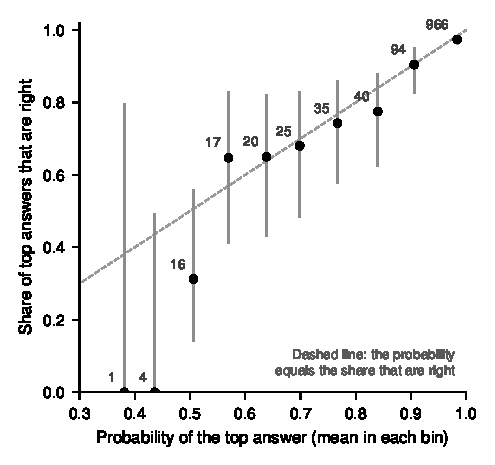
\includegraphics[width=\linewidth]{figures/reliability.pdf}
\end{minipage}\hfill
\begin{minipage}[c]{0.56\textwidth}
\caption{Reliability diagram of v0.5's Evidence Inference 2.0 specialist on the test split (1,218 prompts). The prompts are grouped in the 15 equal-width bins of the reported expected calibration error by the probability of the top answer; each point is a bin's mean probability against the share of its top answers that were right, with the bin's count of prompts and a 95 percent Wilson interval (descriptive). The Wilson intervals treat the prompts as independent, so they are narrower than the article-level intervals used elsewhere. Bins with no prompt are not drawn.}
\label{fig:reliability}
\end{minipage}
\end{figure}

\paragraph{PubMedQA and readmission (descriptive).} On PubMedQA's 500 test items, the PubMedQA specialist's accuracy was 0.7960 (0.7600 to 0.8340) and its log loss 0.5797 (Table~\ref{tab:pubmedqa}). For its answer ``no'', the calibration slope was 1.1869 (1.0296 to 1.4260): the interval excludes 1, so miscalibration was detected, with probabilities less extreme than the outcomes support (registered; descriptive; Appendix~\ref{app:answers}). Against BioGPT-Large-PubMedQA, reported uncalibrated as its primary result (Table~\ref{tab:pubmedqa}), the specialist's log loss was lower by 0.3102 (0.1996 to 0.4219) and its accuracy higher by 0.0440 (0.0139 to 0.0780). Against Gemma 4 31B-it, BioGPT-Large-PubMedQA's log loss was higher by 0.2768 (0.1695 to 0.3925); for accuracy no difference was detected, $-$0.0320 ($-$0.0680 to 0.0040), and the interval excludes a gain for BioGPT-Large-PubMedQA above 0.0040 and a loss above 0.0680 (K5; registered, descriptive). On the 6,998 readmission test encounters, the pool's log loss was 0.8275 against the prior's 0.8861, and its AUROC (area under the receiver operating characteristic curve) for readmission within 30 days was 0.6622 (Table~\ref{tab:readmission}). TabICLv2, a registered candidate member of a new pool, was NOT BUILT because of an error in the project's version check, so the new pool was fitted without it and K6's comparison of TabICLv2 with LightGBM \citep{ke2017} was not computed (Appendix~\ref{app:deviations}). The new pool's out-of-fold log loss, 0.8368, was not below v0.4's pool's, 0.8372, by the 0.002 the rule required, so v0.5 kept v0.4's pool, and K6's difference between the pools is zero. K6's comparisons of two trees refitted with recoded diagnosis fields, neither of them in v0.5's pool, are in Appendix~\ref{app:runs} (registered, descriptive).

\begin{table}[t]
\centering\footnotesize
\caption{PubMedQA, the 500 expert-labeled test items (descriptive: this test split was read in the evaluation of every version). Each cell gives the estimate and its 95 percent interval from 1,000 item resamples; ECE is the expected calibration error. BioGPT-Large-PubMedQA was fine-tuned on sets that hold all 150 validation items, so its uncalibrated probabilities are its primary result and its calibration on those items is secondary.}
\label{tab:pubmedqa}
\begin{tabular}{>{\raggedright\arraybackslash}p{3.0cm}ccccc}
\toprule
System & Accuracy & Macro-F1 & Log loss & Brier score & ECE \\
\midrule
Fiorillo v0.5 (\texttt{s7\_b3}) & \begin{tabular}[t]{@{}c@{}}0.7960\\[-1pt]{\scriptsize (0.7600 to 0.8340)}\end{tabular} & \begin{tabular}[t]{@{}c@{}}0.5698\\[-1pt]{\scriptsize (0.5406 to 0.6039)}\end{tabular} & \begin{tabular}[t]{@{}c@{}}0.5797\\[-1pt]{\scriptsize (0.5070 to 0.6509)}\end{tabular} & \begin{tabular}[t]{@{}c@{}}0.3147\\[-1pt]{\scriptsize (0.2683 to 0.3595)}\end{tabular} & \begin{tabular}[t]{@{}c@{}}0.0401\\[-1pt]{\scriptsize (0.0315 to 0.0800)}\end{tabular} \\[2pt]
Gemma 4 31B-it & \begin{tabular}[t]{@{}c@{}}0.7840\\[-1pt]{\scriptsize (0.7460 to 0.8200)}\end{tabular} & \begin{tabular}[t]{@{}c@{}}0.5862\\[-1pt]{\scriptsize (0.5527 to 0.6252)}\end{tabular} & \begin{tabular}[t]{@{}c@{}}0.6131\\[-1pt]{\scriptsize (0.5309 to 0.6957)}\end{tabular} & \begin{tabular}[t]{@{}c@{}}0.3209\\[-1pt]{\scriptsize (0.2728 to 0.3696)}\end{tabular} & \begin{tabular}[t]{@{}c@{}}0.0575\\[-1pt]{\scriptsize (0.0431 to 0.0970)}\end{tabular} \\[2pt]
BioGPT-Large-PubMedQA, uncalibrated & \begin{tabular}[t]{@{}c@{}}0.7520\\[-1pt]{\scriptsize (0.7120 to 0.7900)}\end{tabular} & \begin{tabular}[t]{@{}c@{}}0.5481\\[-1pt]{\scriptsize (0.5119 to 0.5922)}\end{tabular} & \begin{tabular}[t]{@{}c@{}}0.8899\\[-1pt]{\scriptsize (0.7428 to 1.0347)}\end{tabular} & \begin{tabular}[t]{@{}c@{}}0.4058\\[-1pt]{\scriptsize (0.3462 to 0.4623)}\end{tabular} & \begin{tabular}[t]{@{}c@{}}0.1371\\[-1pt]{\scriptsize (0.1114 to 0.1803)}\end{tabular} \\[2pt]
BioGPT-Large-PubMedQA, calibrated (secondary) & \begin{tabular}[t]{@{}c@{}}0.7380\\[-1pt]{\scriptsize (0.6980 to 0.7761)}\end{tabular} & \begin{tabular}[t]{@{}c@{}}0.5269\\[-1pt]{\scriptsize (0.4963 to 0.5638)}\end{tabular} & \begin{tabular}[t]{@{}c@{}}0.7340\\[-1pt]{\scriptsize (0.6341 to 0.8367)}\end{tabular} & \begin{tabular}[t]{@{}c@{}}0.3886\\[-1pt]{\scriptsize (0.3352 to 0.4389)}\end{tabular} & \begin{tabular}[t]{@{}c@{}}0.0876\\[-1pt]{\scriptsize (0.0667 to 0.1299)}\end{tabular} \\[2pt]
Prior & \begin{tabular}[t]{@{}c@{}}0.5520\\[-1pt]{\scriptsize (0.5080 to 0.5940)}\end{tabular} & \begin{tabular}[t]{@{}c@{}}0.2371\\[-1pt]{\scriptsize (0.2246 to 0.2484)}\end{tabular} & \begin{tabular}[t]{@{}c@{}}1.1593\\[-1pt]{\scriptsize (1.0401 to 1.2920)}\end{tabular} & \begin{tabular}[t]{@{}c@{}}0.5855\\[-1pt]{\scriptsize (0.5503 to 0.6208)}\end{tabular} & \begin{tabular}[t]{@{}c@{}}0.0646\\[-1pt]{\scriptsize (0.0226 to 0.1086)}\end{tabular} \\[2pt]
\bottomrule
\end{tabular}

\end{table}

\begin{table}[t]
\centering\footnotesize
\caption{Readmission on the University of California, Irvine, Diabetes 130-US hospitals data, the 6,998 test encounters (descriptive: this test split was read in the evaluation of every version). Each cell gives the estimate and its 95 percent interval from 1,000 item resamples. ECE is the expected calibration error, whose percentile interval can lie above its estimate, since the ECE is biased upward in resamples; AUROC is the area under the receiver operating characteristic curve; it and the calibration intercept and slope are for readmission within 30 days against the rest. The calibration slope is not computed for the prior, whose prediction is the same for every encounter.}
\label{tab:readmission}
\setlength{\tabcolsep}{3.5pt}
\begin{tabular}{>{\raggedright\arraybackslash}p{2.0cm}cccccc}
\toprule
System & Log loss & ECE & Accuracy & \shortstack{AUROC,\\ 30 days} & \shortstack{Calibration\\ intercept, 30 days} & \shortstack{Calibration\\ slope, 30 days} \\
\midrule
Fiorillo v0.5 (tree pool) & \begin{tabular}[t]{@{}c@{}}0.8275\\[-1pt]{\scriptsize (0.8132 to 0.8411)}\end{tabular} & \begin{tabular}[t]{@{}c@{}}0.0066\\[-1pt]{\scriptsize (0.0085 to 0.0225)}\end{tabular} & \begin{tabular}[t]{@{}c@{}}0.6157\\[-1pt]{\scriptsize (0.6042 to 0.6269)}\end{tabular} & \begin{tabular}[t]{@{}c@{}}0.6622\\[-1pt]{\scriptsize (0.6394 to 0.6855)}\end{tabular} & \begin{tabular}[t]{@{}c@{}}$-$0.0192\\[-1pt]{\scriptsize ($-$0.1031 to 0.0646)}\end{tabular} & \begin{tabular}[t]{@{}c@{}}1.0493\\[-1pt]{\scriptsize (0.9108 to 1.1940)}\end{tabular} \\[2pt]
Prior & \begin{tabular}[t]{@{}c@{}}0.8861\\[-1pt]{\scriptsize (0.8734 to 0.8984)}\end{tabular} & \begin{tabular}[t]{@{}c@{}}0.0017\\[-1pt]{\scriptsize (0.0002 to 0.0127)}\end{tabular} & \begin{tabular}[t]{@{}c@{}}0.5942\\[-1pt]{\scriptsize (0.5829 to 0.6047)}\end{tabular} & \begin{tabular}[t]{@{}c@{}}0.5000\\[-1pt]{\scriptsize (0.5000 to 0.5000)}\end{tabular} & \begin{tabular}[t]{@{}c@{}}$-$0.0299\\[-1pt]{\scriptsize ($-$0.1120 to 0.0536)}\end{tabular} & not computed \\[2pt]
\bottomrule
\end{tabular}

\end{table}

\paragraph{The other registered comparisons.} On the clean validation prompts, the longer input's two-run average scored a lower log loss than the base recipe's, by 0.0286 (0.0097 to 0.0496); for the other candidates no difference was detected (K3, registered; Appendix~\ref{app:runs} gives their intervals and what they exclude). On test, v0.5's specialist minus the base recipe's three-run average (\sysname{s9\_b}) gave a log-loss difference of 0.0000 ($-$0.0202 to 0.0174): no difference was detected, and the interval excludes a gain above 0.0202 and a loss above 0.0174 (K3, registered). The weight average's log loss was higher than the three runs' probability average by 0.0048 (0.0010 to 0.0092) (K8; registered, descriptive). The four-family calibration chose the same family as v0.4's two-family rule, so K9's difference is zero (registered, descriptive). Averaging each answer with the answer to the exchanged prompt raised log loss by 0.0922 (0.0672 to 0.1206) and ECE by 0.0481 (0.0259 to 0.0602) (K10; registered, descriptive).

\paragraph{The usage check.} I ran the release as a user would, at the fixed revision that the statements give: its own inference script on a MacBook Pro with an Apple M5 chip, under macOS, with each question's records as a file of their own; the readers ran on the laptop's graphics processing unit and the readmission trees on its central processing unit. Rules fixed before the check's first run compared the answers with the evaluated test predictions: readmission passes when every probability is within 0.0001 of the evaluated one, and EI and PubMedQA pass when no top answer changes on a record whose evaluated top probability is at least 0.6 and the mean absolute difference over all records and answers is at most 0.02. All three passed. On the 6,998 readmission encounters, the largest difference was below one in ten million. On the 500 PubMedQA items, the mean absolute difference was 0.0013 and the largest 0.0159; on 60 EI prompts drawn at random from the 1,218, each with the input it was evaluated on, the mean was 0.0028 and the largest 0.0459. No top answer changed on either. The EI records hold each article as the evaluated predictions read it, already cut to 6,144 tokens, so the check does not cover the passage selection of a whole article.

% SECTION: reading
\section{Does the model read the article?}
\label{sec:reading}

EI's labels have been public since 2019, the trials' results are in PubMed, and the pretraining text of Qwen3 and Gemma 4 is not published. A model could answer some prompts from what it read before this project rather than from the article in front of it. The reading checks ask the specialists the test prompts with no article, with the title alone, and with the intervention and the comparator exchanged (registered as K4); their readings were fixed in the update before they ran (Table~\ref{tab:reading}, Figure~\ref{fig:reading}).

\begin{table}[t]
\centering\footnotesize
\caption{The reading checks on Evidence Inference 2.0's test split (registered as K4, with readings fixed in advance). Each cell gives the estimate and its 95 percent interval from 1,000 article resamples. The title input leaves out the 9 prompts whose article gives no title (derived); the title's difference is computed on the prompts in both inputs. ``Direction answers'' are ``significantly increased'' and ``significantly decreased''; for them the exchanged prompt's expected answer is the other direction.}
\label{tab:reading}
\begin{tabular}{>{\raggedright\arraybackslash}p{5.4cm}rcrc}
\toprule
Statistic & Prompts & v0.4 (\texttt{s8\_ei}) & Prompts & v0.5 (\texttt{s9\_ei\_wavg}) \\
\midrule
\multicolumn{5}{@{}l}{\textit{No article}} \\[1pt]
Accuracy & 1,218 & 0.5090 {\scriptsize (0.4779 to 0.5439)} & 1,218 & 0.5156 {\scriptsize (0.4874 to 0.5494)} \\
Macro-F1 & 1,218 & 0.4289 {\scriptsize (0.3941 to 0.4634)} & 1,218 & 0.4384 {\scriptsize (0.4085 to 0.4726)} \\
Agreement with the whole-article answer & 1,218 & 0.5140 {\scriptsize (0.4812 to 0.5473)} & 1,218 & 0.5238 {\scriptsize (0.4955 to 0.5571)} \\
\multicolumn{5}{@{}l}{\textit{Title only}} \\[1pt]
Accuracy & 1,209 & 0.5715 {\scriptsize (0.5346 to 0.6065)} & 1,209 & 0.5715 {\scriptsize (0.5389 to 0.6041)} \\
Macro-F1 & 1,209 & 0.5338 {\scriptsize (0.4964 to 0.5733)} & 1,209 & 0.5327 {\scriptsize (0.4995 to 0.5692)} \\
Agreement with the whole-article answer & 1,209 & 0.5682 {\scriptsize (0.5343 to 0.6027)} & 1,209 & 0.5782 {\scriptsize (0.5471 to 0.6108)} \\
Macro-F1, no article, on the same prompts & 1,209 & 0.4314 {\scriptsize (0.3967 to 0.4650)} & 1,209 & 0.4388 {\scriptsize (0.4076 to 0.4723)} \\
Macro-F1, title only minus no article & 1,209 & 0.1024 {\scriptsize (0.0736 to 0.1331)} & 1,209 & 0.0939 {\scriptsize (0.0655 to 0.1234)} \\
\multicolumn{5}{@{}l}{\textit{Intervention and comparator exchanged}} \\[1pt]
Accuracy against the exchanged answers & 1,218 & 0.8103 {\scriptsize (0.7802 to 0.8400)} & 1,218 & 0.7808 {\scriptsize (0.7493 to 0.8117)} \\
Macro-F1 against the exchanged answers & 1,218 & 0.7958 {\scriptsize (0.7633 to 0.8283)} & 1,218 & 0.7600 {\scriptsize (0.7268 to 0.7946)} \\
Share of direction answers that exchange & 703 & 0.7226 {\scriptsize (0.6765 to 0.7714)} & 699 & 0.6652 {\scriptsize (0.6208 to 0.7157)} \\
Share of no-difference answers that stay & 515 & 0.9806 {\scriptsize (0.9657 to 0.9931)} & 519 & 0.9672 {\scriptsize (0.9477 to 0.9841)} \\
\multicolumn{5}{@{}l}{\textit{Exchanged, on the prompts whose comparator is a time point or a baseline}} \\[1pt]
Share of direction answers that exchange & 38 & 0.1316 {\scriptsize (0.0250 to 0.2632)} & 37 & 0.2162 {\scriptsize (0.0857 to 0.3439)} \\
Share of no-difference answers that stay & 10 & 1.0000 {\scriptsize (1.0000 to 1.0000)} & 11 & 1.0000 {\scriptsize (1.0000 to 1.0000)} \\
\bottomrule
\end{tabular}

\end{table}

\begin{figure}[t]
\begin{minipage}[c]{0.46\textwidth}
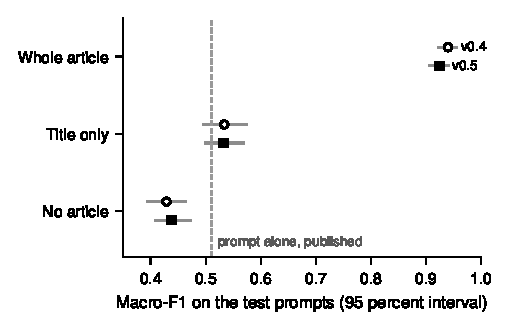
\includegraphics[width=\linewidth]{figures/reading.pdf}
\end{minipage}\hfill
\begin{minipage}[c]{0.50\textwidth}
\caption{Macro-F1 of v0.4's (open circles) and v0.5's (filled squares) Evidence Inference 2.0 specialists on the test prompts, with the whole article (1,218 prompts), the title only (1,209) and no article (1,218), each with its 95 percent interval from 1,000 article resamples. The dashed line is the macro-F1 that \citet{deyoung2020} report for a classifier given the prompt alone, 0.511 (descriptive: a different model, scored and counted as that paper did).}
\label{fig:reading}
\end{minipage}
\end{figure}

\paragraph{No article.} With the article set to empty text, v0.5's macro-F1 was 0.4384 (0.4085 to 0.4726), and v0.4's 0.4289 (0.3941 to 0.4634), against 0.1976 (0.1855 to 0.2095) for the training split's answer shares, a reference the update fixed. The fixed reading for a macro-F1 at or below 0.60 is ``its answers depend on the article's text'', and it applies to both. Both intervals lie below the 0.511 that \citet{deyoung2020} report for a classifier trained to answer from the prompt alone, a different model on their own scoring (descriptive).

\paragraph{Title only.} On the 1,209 prompts whose article gives a title, the title alone raised v0.5's macro-F1 over no article, on the same prompts, by 0.0939 (0.0655 to 0.1234), and v0.4's by 0.1024 (0.0736 to 0.1331). The intervals lie wholly above 0.05, so the fixed reading applies to both: ``the title adds information about the result: a title can state the result, or the model may recall the trial, and these checks cannot tell them apart''. \citet{windisch2026} report that frontier models reached an accuracy of 0.79 to 0.88 from titles alone on 250 oncology trials, on a two-answer task whose majority class was 0.584.

\paragraph{Intervention and comparator exchanged.} When the intervention and the comparator are exchanged, a model that follows the comparison as written should exchange its ``increased'' and ``decreased'' answers. v0.5 exchanged 0.6652 (0.6208 to 0.7157) of its direction answers, and v0.4 0.7226 (0.6765 to 0.7714). Where the comparator is a time point or a baseline, v0.5 exchanged 0.2162 of its 37 direction answers. Against the exchanged answers, v0.5's accuracy was 0.7808 (0.7493 to 0.8117) and v0.4's 0.8103 (0.7802 to 0.8400), which the fixed reading calls ``partly'' for both. This is a weakness: the specialist often keeps its direction when the comparison is reversed. The fix to test (I-97 in the project's register of ideas) is to train on prompts whose comparator is a time point or a baseline together with their exchanged copies, or with a training term that asks the answer to an exchanged prompt to be the exchange of the original answer. Exchanged copies of all training prompts were a candidate in the recipe rule and did not pass on validation, and averaging each answer with the answer to the exchanged prompt made log loss worse (K10, Section~\ref{sec:results}).

% SECTION: license
\section{What training on openly licensed articles cost}
\label{sec:license}

K2 compares training on the clean articles alone with training on all of them (registered; descriptive). The same recipe as v0.4, trained on the 1,431 clean training articles and calibrated on the 654 clean validation prompts (\sysname{s9\_b}, three runs averaged), had a lower accuracy than v0.4's specialist, trained on all 2,657 and calibrated on all 1,237 validation prompts, by 0.0123 (0.0034 to 0.0207), and a higher log loss by 0.0170 (0.0058 to 0.0284) (Table~\ref{tab:k2}). Both chose temperature scaling, which does not change the top answer, so the accuracy difference comes from training alone, while the log-loss difference also reflects the different calibration prompts. v0.5's specialist, which also uses the longer input, had a lower accuracy than v0.4's by 0.0140 (0.0025 to 0.0245); for log loss no difference was detected, 0.0169 ($-$0.0095 to 0.0397), and the interval excludes a gain for v0.5 above 0.0095 and a loss above 0.0397.

\begin{table}[t]
\centering\footnotesize
\caption{What the license cost (K2; registered, descriptive): each system minus v0.4's specialist on Evidence Inference 2.0's test split (1,218 prompts in 333 articles), with 95 percent intervals from 1,000 article resamples. Each is calibrated on validation: the clean systems on the 654 clean validation prompts, v0.4's on all 1,237. ECE is the expected calibration error. \textsuperscript{\dag}No difference was detected: the interval includes zero.}
\label{tab:k2}
\setlength{\tabcolsep}{3.5pt}
\begin{tabular}{>{\raggedright\arraybackslash}p{3.0cm}ccccc}
\toprule
Minus v0.4 (\texttt{s8\_ei}) & Accuracy & Macro-F1 & Log loss & Brier score & ECE \\
\midrule
Same recipe, clean articles only (\texttt{s9\_b}) & \begin{tabular}[t]{@{}c@{}}$-$0.0123\\[-1pt]{\scriptsize ($-$0.0207 to $-$0.0034)}\end{tabular} & \begin{tabular}[t]{@{}c@{}}$-$0.0133\\[-1pt]{\scriptsize ($-$0.0226 to $-$0.0041)}\end{tabular} & \begin{tabular}[t]{@{}c@{}}0.0170\\[-1pt]{\scriptsize (0.0058 to 0.0284)}\end{tabular} & \begin{tabular}[t]{@{}c@{}}0.0106\\[-1pt]{\scriptsize (0.0037 to 0.0174)}\end{tabular} & \begin{tabular}[t]{@{}c@{}}0.0007\textsuperscript{\dag}\\[-1pt]{\scriptsize ($-$0.0105 to 0.0102)}\end{tabular} \\[2pt]
Fiorillo v0.5 (\texttt{s9\_ei\_wavg}) & \begin{tabular}[t]{@{}c@{}}$-$0.0140\\[-1pt]{\scriptsize ($-$0.0245 to $-$0.0025)}\end{tabular} & \begin{tabular}[t]{@{}c@{}}$-$0.0152\\[-1pt]{\scriptsize ($-$0.0261 to $-$0.0036)}\end{tabular} & \begin{tabular}[t]{@{}c@{}}0.0169\textsuperscript{\dag}\\[-1pt]{\scriptsize ($-$0.0095 to 0.0397)}\end{tabular} & \begin{tabular}[t]{@{}c@{}}0.0100\textsuperscript{\dag}\\[-1pt]{\scriptsize ($-$0.0055 to 0.0231)}\end{tabular} & \begin{tabular}[t]{@{}c@{}}0.0048\textsuperscript{\dag}\\[-1pt]{\scriptsize ($-$0.0093 to 0.0144)}\end{tabular} \\[2pt]
\bottomrule
\end{tabular}

\end{table}

% SECTION: handoff
\section{Handing questions to a larger model}
\label{sec:handoff}

K7 asks what happens when the specialist's least confident answers go to Gemma 4 31B-it reading the same input (registered; secondary and descriptive); v0.5 itself hands nothing off. Table~\ref{tab:handoff} gives the combined accuracy at the four registered rates for five ways of choosing the prompts handed off. With the confidence rule, which hands off the least confident answers, the combined accuracy was 0.9335 with 10 percent handed off and 0.8768 with 50 percent, against 0.9269 for v0.5 alone and 0.8752 for the large model alone; the oracle's bound was 0.9573. The results files hold no interval for the combined system minus v0.5 alone, so no difference from v0.5 alone is claimed. The specialist was wrong where the large model was right on 37 of the 1,218 test prompts (a share of 0.0304), and right where the large model was wrong on 100: these few prompts bound what any rule could gain and leave a learned rule few cases to learn from. Against the confidence rule, no difference was detected for the rule learned on validation at any rate, and each interval excludes a gain larger than 0.0041 and a loss larger than 0.0048 in combined accuracy. The area under the specialist's risk-coverage curve (AURC) was 0.0128 (0.0082 to 0.0182), its excess over a perfect ranking of the same answers 0.0100 (0.0064 to 0.0145), and the area under the generalized risk-coverage curve 0.0105 (0.0069 to 0.0147); the curves are not drawn, since Table~\ref{tab:handoff} gives the registered rates and the curves at every 5 percent are in the results files. For v0.4's specialist with the large model on 4,096-token inputs, the combined accuracy at 10 percent was 0.9294 against 0.9409 alone; for the PubMedQA specialist, 0.8000 against 0.7960 alone.

\begin{table}[t]
\centering\scriptsize
\caption{K7 (registered; secondary and descriptive): the combined accuracy of v0.5's Evidence Inference 2.0 specialist and Gemma 4 31B-it, reading the same input, when a share of the 1,218 test prompts is handed to the large model, with 95 percent intervals from 1,000 article resamples. The learned rule was fitted and frozen on validation. Random gives the expected value of random hand-off. The large model's confidence hands off first the items on which the large model's own top probability is highest, which needs its answer on every item. The oracle hands off the items the specialist gets wrong and the large model gets right, which bounds any rule. v0.5 alone: 0.9269; the large model alone: 0.8752.}
\label{tab:handoff}
\begin{tabular}{lrccccc}
\toprule
Handed off & Prompts & Confidence rule & Learned rule & Random (expected) & \shortstack{Large model's\\ confidence} & Oracle \\
\midrule
10 percent & 121 & \begin{tabular}[t]{@{}c@{}}0.9335\\[-1pt]{\scriptsize (0.9160 to 0.9492)}\end{tabular} & \begin{tabular}[t]{@{}c@{}}0.9335\\[-1pt]{\scriptsize (0.9150 to 0.9493)}\end{tabular} & \begin{tabular}[t]{@{}c@{}}0.9218\\[-1pt]{\scriptsize (0.9040 to 0.9369)}\end{tabular} & \begin{tabular}[t]{@{}c@{}}0.9269\\[-1pt]{\scriptsize (0.9097 to 0.9428)}\end{tabular} & \begin{tabular}[t]{@{}c@{}}0.9573\\[-1pt]{\scriptsize (0.9442 to 0.9693)}\end{tabular} \\[2pt]
20 percent & 243 & \begin{tabular}[t]{@{}c@{}}0.9171\\[-1pt]{\scriptsize (0.8986 to 0.9328)}\end{tabular} & \begin{tabular}[t]{@{}c@{}}0.9163\\[-1pt]{\scriptsize (0.8993 to 0.9336)}\end{tabular} & \begin{tabular}[t]{@{}c@{}}0.9166\\[-1pt]{\scriptsize (0.8988 to 0.9322)}\end{tabular} & \begin{tabular}[t]{@{}c@{}}0.9261\\[-1pt]{\scriptsize (0.9076 to 0.9430)}\end{tabular} & \begin{tabular}[t]{@{}c@{}}0.9573\\[-1pt]{\scriptsize (0.9442 to 0.9693)}\end{tabular} \\[2pt]
30 percent & 365 & \begin{tabular}[t]{@{}c@{}}0.8966\\[-1pt]{\scriptsize (0.8751 to 0.9173)}\end{tabular} & \begin{tabular}[t]{@{}c@{}}0.8966\\[-1pt]{\scriptsize (0.8750 to 0.9170)}\end{tabular} & \begin{tabular}[t]{@{}c@{}}0.9114\\[-1pt]{\scriptsize (0.8935 to 0.9276)}\end{tabular} & \begin{tabular}[t]{@{}c@{}}0.9245\\[-1pt]{\scriptsize (0.9055 to 0.9423)}\end{tabular} & \begin{tabular}[t]{@{}c@{}}0.9573\\[-1pt]{\scriptsize (0.9442 to 0.9693)}\end{tabular} \\[2pt]
50 percent & 609 & \begin{tabular}[t]{@{}c@{}}0.8768\\[-1pt]{\scriptsize (0.8535 to 0.9013)}\end{tabular} & \begin{tabular}[t]{@{}c@{}}0.8777\\[-1pt]{\scriptsize (0.8532 to 0.9014)}\end{tabular} & \begin{tabular}[t]{@{}c@{}}0.9011\\[-1pt]{\scriptsize (0.8821 to 0.9182)}\end{tabular} & \begin{tabular}[t]{@{}c@{}}0.9261\\[-1pt]{\scriptsize (0.9073 to 0.9441)}\end{tabular} & \begin{tabular}[t]{@{}c@{}}0.9573\\[-1pt]{\scriptsize (0.9442 to 0.9693)}\end{tabular} \\[2pt]
\bottomrule
\end{tabular}

\end{table}

At the rate of the rented graphics processing unit (GPU), \$3.52 an hour, 1,000 EI questions cost \$0.297 of GPU time with v0.5's specialist and \$2.443 with Gemma 4 31B-it, from the time each took on the GPU in the test predictions (derived; Appendix~\ref{app:cost}).

% SECTION: limits
\section{Limitations}
\label{sec:limits}

\begin{itemize}\setlength{\itemsep}{1pt}
\item One question type for trials was tested: one comparison in a randomized trial's article, in English, with the article cut to 6,144 tokens. Other questions, wordings and kinds of document are untested and uncalibrated.
\item EI's test split has been read for v0.4's bar and checks, for the reading checks of v0.4's specialist and for v0.5's bar; PubMedQA's and readmission's test splits were read in every version.
\item The pretraining text of Qwen3 and Gemma 4 is not published and may include PMC articles (EI's articles come from PMC), EI's repository (public since 2019), PubMedQA and the UCI readmission data; this would favor both models. EI's test labels are public, so no evaluation of EI can be blind. In a check that was not registered (descriptive), 10 EI test articles (37 prompts) shared sentences with PubMedQA abstracts that the PubMedQA specialist, from whose weights the EI specialists started, had read in training; v0.4's specialist's accuracy on them was 0.8378 (0.6667 to 0.9445), and no difference from the other prompts was detected, $-$0.1063 ($-$0.2817 to 0.0051), the interval excluding a gain above 0.0051 and a loss above 0.2817.
\item The title effect is unresolved, and the specialist often keeps its direction when the intervention and comparator are exchanged (Section~\ref{sec:reading}).
\item The released specialist's EI training used only clean articles, with the two exceptions of Section~\ref{sec:data}: the passage selection's word statistics, counted over all training articles, and its start from the PubMedQA specialist, whose abstracts' licenses were not checked one by one.
\item The large model is a reference that was not trained on the task; it ran zero-shot with thinking off, its answers read from its next token's letter probabilities, and its prompt and that reading were fixed, not tuned.
\item Fiorillo is a research model and is not for clinical use. No person was recruited for this work.
\end{itemize}

% SECTION: discussion
\section{Discussion}
\label{sec:discussion}

A 4-billion-parameter open model, fine-tuned for EI only on articles whose own licenses allow reuse (it started from a PubMedQA specialist whose abstracts' licenses were not checked one by one), met a bar fixed in advance on EI's test split, the second bar judged on that split. Its stated probabilities matched how often it was right within the registered limit: its expected calibration error was 0.0168 against 0.05, and no miscalibration of any answer was detected by the per-answer calibration slopes and intercepts (Appendix~\ref{app:answers}). These figures hold as far as EI's test split represents a reader's trials.

What the test does not show is how much of the accuracy comes from reading the article and how much from what the base model read before. The answers depend on the article, but the title adds information, and the checks here cannot separate a title that states the result from recall of the trial. Two results would change that reading: a test on trials posted after the base model's release, where recall is not possible (I-42 and I-94 in the project's register of ideas), and a specialist that follows an exchanged comparison (I-97).

The license recheck had a measurable cost: the same recipe was less accurate when it learned only from clean articles (Table~\ref{tab:k2}; descriptive). The release makes that trade explicit, and its NOTICE file credits each of the 1,610 clean training and validation articles (derived) with its identifier, license and citation.

% SECTION: statements
\section*{Statements}
\label{sec:statements}

\paragraph{Conflicts of interest.} I may later build a company on this model.

\paragraph{Funding.} None. I paid for the computing myself.

\paragraph{Ethics.} This work used public, de-identified data and published articles only. No person was recruited or contacted.

\paragraph{Data and code availability.} The release: Fiorillo v0.5 on Hugging Face, digital object identifier (DOI) \doi{10.57967/hf/10722} \citep{fiorillo05}, under the Apache License 2.0, with its model card, its inference script and a NOTICE file that credits each clean article with its identifier, license and citation. Its revision \idn{0058ed7} differs from the revision the DOI records, \idn{56e5944}, only in how the script loads its libraries, so that each question runs on macOS when its records are a file of their own, and in a note in the model card. The project's earlier reader: DOI \doi{10.57967/hf/10658} \citep{reader1}. The registration and its update: \mbox{\url{https://osf.io/kaxmn/}} \citep{osfreg}. The code, the results files and this paper's sources: \mbox{\url{https://github.com/johann-e-li/fiorillo}}, under the Apache License 2.0.

\paragraph{Use of artificial intelligence tools.} Claude, by Anthropic, wrote much of the code, ran the analyses with me and drafted the text. I reviewed every part and take responsibility for all of it. Artificial intelligence (AI) tools are not authors.

\begin{thebibliography}{29}
\providecommand{\natexlab}[1]{#1}

\bibitem[Brier(1950)]{brier1950}
Glenn W. Brier.
\newblock Verification of forecasts expressed in terms of probability.
\newblock \emph{Monthly Weather Review}, volume 78, issue 1, pages 1 to 3, 1950.
\newblock \doi{10.1175/1520-0493(1950)078<0001:VOFEIT>2.0.CO;2}.

\bibitem[Buchmann et~al.(2024a)Buchmann, Eichler, Bodensohn, Kuznetsov, and Gurevych]{buchmann2024structure}
Jan Buchmann, Max Eichler, Jan-Micha Bodensohn, Ilia Kuznetsov, and Iryna Gurevych.
\newblock Document structure in long document transformers.
\newblock In \emph{Proceedings of the 18th Conference of the European Chapter of the Association for Computational Linguistics (Volume 1: Long Papers)}, pages 1056 to 1073, St.\ Julian's, Malta, 2024a.
\newblock \doi{10.18653/v1/2024.eacl-long.64}.

\bibitem[Buchmann et~al.(2024b)Buchmann, Liu, and Gurevych]{buchmann2024lab}
Jan Buchmann, Xiao Liu, and Iryna Gurevych.
\newblock Attribute or abstain: Large language models as long document assistants.
\newblock In \emph{Proceedings of the 2024 Conference on Empirical Methods in Natural Language Processing}, pages 8113 to 8140, Miami, Florida, USA, 2024b.
\newblock \doi{10.18653/v1/2024.emnlp-main.463}.

\bibitem[Chen and Guestrin(2016)]{chen2016}
Tianqi Chen and Carlos Guestrin.
\newblock {XGBoost}: A scalable tree boosting system.
\newblock In \emph{Proceedings of the 22nd ACM SIGKDD International Conference on Knowledge Discovery and Data Mining}, pages 785 to 794, San Francisco, California, USA, 2016.
\newblock \doi{10.1145/2939672.2939785}.

\bibitem[DeYoung et~al.(2020)DeYoung, Lehman, Nye, Marshall, and Wallace]{deyoung2020}
Jay DeYoung, Eric Lehman, Benjamin Nye, Iain Marshall, and Byron C. Wallace.
\newblock Evidence Inference 2.0: More data, better models.
\newblock In \emph{Proceedings of the 19th SIGBioMed Workshop on Biomedical Language Processing}, pages 123 to 132, online, 2020. Association for Computational Linguistics.
\newblock \doi{10.18653/v1/2020.bionlp-1.13}.

\bibitem[Geifman and El-Yaniv(2017)]{geifman2017}
Yonatan Geifman and Ran El-Yaniv.
\newblock Selective classification for deep neural networks.
\newblock In \emph{Advances in Neural Information Processing Systems 30}, 2017.
\newblock \url{https://proceedings.neurips.cc/paper_files/paper/2017/hash/4a8423d5e91fda00bb7e46540e2b0cf1-Abstract.html}.

\bibitem[Gemma~Team(2026)]{gemma4}
Gemma Team.
\newblock Gemma 4 technical report.
\newblock arXiv:2607.02770, 2026.
\newblock \doi{10.48550/arXiv.2607.02770}. Checkpoint: \url{https://huggingface.co/google/gemma-4-31B-it}.

\bibitem[Gorenshtein et~al.(2026)Gorenshtein, Omar, Barash, Kruskal, Ahmed, Brook, Illigens, Nadkarni, and Klang]{gorenshtein2026}
Alon Gorenshtein, Mahmud Omar, Yiftach Barash, Jonathan B. Kruskal, Muneeb Ahmed, Olga R. Brook, Ben Illigens, Girish N. Nadkarni, and Eyal Klang.
\newblock Small language models in clinical medicine: a systematic review of performance, safety, and deployment feasibility.
\newblock \emph{Journal of the American Medical Informatics Association}, advance article ocag164, 2026.
\newblock \doi{10.1093/jamia/ocag164}.

\bibitem[Guo et~al.(2017)Guo, Pleiss, Sun, and Weinberger]{guo2017}
Chuan Guo, Geoff Pleiss, Yu Sun, and Kilian Q. Weinberger.
\newblock On calibration of modern neural networks.
\newblock In \emph{Proceedings of the 34th International Conference on Machine Learning}, volume 70 of \emph{Proceedings of Machine Learning Research}, pages 1321 to 1330, 2017.
\newblock \url{https://proceedings.mlr.press/v70/guo17a.html}.

\bibitem[Hu et~al.(2022)Hu, Shen, Wallis, Allen-Zhu, Li, Wang, Wang, and Chen]{hu2022}
Edward J. Hu, Yelong Shen, Phillip Wallis, Zeyuan Allen-Zhu, Yuanzhi Li, Shean Wang, Lu Wang, and Weizhu Chen.
\newblock {LoRA}: Low-rank adaptation of large language models.
\newblock In \emph{International Conference on Learning Representations}, 2022.
\newblock \url{https://iclr.cc/virtual/2022/poster/6319}.

\bibitem[Jin et~al.(2019)Jin, Dhingra, Liu, Cohen, and Lu]{jin2019}
Qiao Jin, Bhuwan Dhingra, Zhengping Liu, William Cohen, and Xinghua Lu.
\newblock {PubMedQA}: A dataset for biomedical research question answering.
\newblock In \emph{Proceedings of the 2019 Conference on Empirical Methods in Natural Language Processing and the 9th International Joint Conference on Natural Language Processing}, pages 2567 to 2577, Hong Kong, China, 2019.
\newblock \doi{10.18653/v1/D19-1259}.

\bibitem[Ke et~al.(2017)Ke, Meng, Finley, Wang, Chen, Ma, Ye, and Liu]{ke2017}
Guolin Ke, Qi Meng, Thomas Finley, Taifeng Wang, Wei Chen, Weidong Ma, Qiwei Ye, and Tie-Yan Liu.
\newblock {LightGBM}: A highly efficient gradient boosting decision tree.
\newblock In \emph{Advances in Neural Information Processing Systems 30}, 2017.
\newblock \url{https://proceedings.neurips.cc/paper_files/paper/2017/hash/6449f44a102fde848669bdd9eb6b76fa-Abstract.html}.

\bibitem[Kull et~al.(2019)Kull, Perello~Nieto, K{\"a}ngsepp, Silva~Filho, Song, and Flach]{kull2019}
Meelis Kull, Miquel Perello Nieto, Markus K{\"a}ngsepp, Telmo Silva Filho, Hao Song, and Peter Flach.
\newblock Beyond temperature scaling: Obtaining well-calibrated multi-class probabilities with {Dirichlet} calibration.
\newblock In \emph{Advances in Neural Information Processing Systems 32}, 2019.
\newblock \url{https://proceedings.neurips.cc/paper_files/paper/2019/hash/8ca01ea920679a0fe3728441494041b9-Abstract.html}.

\bibitem[Lehman et~al.(2019)Lehman, DeYoung, Barzilay, and Wallace]{lehman2019}
Eric Lehman, Jay DeYoung, Regina Barzilay, and Byron C. Wallace.
\newblock Inferring which medical treatments work from reports of clinical trials.
\newblock In \emph{Proceedings of the 2019 Conference of the North American Chapter of the Association for Computational Linguistics: Human Language Technologies, Volume 1 (Long and Short Papers)}, pages 3705 to 3717, Minneapolis, Minnesota, 2019.
\newblock \doi{10.18653/v1/N19-1371}.

\bibitem[Li(2026a)]{osfreg}
Johann Emmanuel Li.
\newblock Fiorillo v0.4 against Gemma 4 31B-it on Evidence Inference 2.0: a test fixed before any test prediction.
\newblock OSF Preregistration, OSF Registries, registered 1 October 2026, with its update of 1 October 2026.
\newblock \doi{10.17605/OSF.IO/KAXMN}.

\bibitem[Li(2026b)]{reader1}
Johann Li.
\newblock fiorillo-reader-v1.
\newblock Hugging Face, model, version c92dc7a, 2026.
\newblock \doi{10.57967/hf/10658}.

\bibitem[Li(2026c)]{fiorillo05}
Johann Li.
\newblock fiorillo-v0.5.
\newblock Hugging Face, model, version 56e5944, 2026.
\newblock \doi{10.57967/hf/10722}.

\bibitem[Luo et~al.(2022)Luo, Sun, Xia, Qin, Zhang, Poon, and Liu]{luo2022}
Renqian Luo, Liai Sun, Yingce Xia, Tao Qin, Sheng Zhang, Hoifung Poon, and Tie-Yan Liu.
\newblock {BioGPT}: generative pre-trained transformer for biomedical text generation and mining.
\newblock \emph{Briefings in Bioinformatics}, volume 23, issue 6, article bbac409, 2022.
\newblock \doi{10.1093/bib/bbac409}.

\bibitem[Marshall et~al.(2020)Marshall, Nye, Kuiper, Noel-Storr, Marshall, Maclean, Soboczenski, Nenkova, Thomas, and Wallace]{marshall2020}
Iain J. Marshall, Benjamin Nye, Jo{\"e}l Kuiper, Anna Noel-Storr, Rachel Marshall, Rory Maclean, Frank Soboczenski, Ani Nenkova, James Thomas, and Byron C. Wallace.
\newblock Trialstreamer: A living, automatically updated database of clinical trial reports.
\newblock \emph{Journal of the American Medical Informatics Association}, volume 27, issue 12, pages 1903 to 1912, 2020.
\newblock \doi{10.1093/jamia/ocaa163}.

\bibitem[Naeini et~al.(2015)Naeini, Cooper, and Hauskrecht]{naeini2015}
Mahdi Pakdaman Naeini, Gregory F. Cooper, and Milos Hauskrecht.
\newblock Obtaining well calibrated probabilities using {Bayesian} binning.
\newblock In \emph{Proceedings of the AAAI Conference on Artificial Intelligence}, volume 29, issue 1, pages 2901 to 2907, 2015.
\newblock \doi{10.1609/aaai.v29i1.9602}.

\bibitem[Prokhorenkova et~al.(2018)Prokhorenkova, Gusev, Vorobev, Dorogush, and Gulin]{prokhorenkova2018}
Liudmila Prokhorenkova, Gleb Gusev, Aleksandr Vorobev, Anna Veronika Dorogush, and Andrey Gulin.
\newblock {CatBoost}: unbiased boosting with categorical features.
\newblock In \emph{Advances in Neural Information Processing Systems 31}, 2018.
\newblock \url{https://proceedings.neurips.cc/paper_files/paper/2018/hash/14491b756b3a51daac41c24863285549-Abstract.html}.

\bibitem[Robertson and Zaragoza(2009)]{robertson2009}
Stephen Robertson and Hugo Zaragoza.
\newblock The probabilistic relevance framework: {BM25} and beyond.
\newblock \emph{Foundations and Trends in Information Retrieval}, volume 3, number 4, pages 333 to 389, 2009.
\newblock \doi{10.1561/1500000019}.

\bibitem[Sainz et~al.(2023)Sainz, Campos, Garc{\'i}a-Ferrero, Etxaniz, Lopez~de Lacalle, and Agirre]{sainz2023}
Oscar Sainz, Jon Campos, Iker Garc{\'i}a-Ferrero, Julen Etxaniz, Oier Lopez de Lacalle, and Eneko Agirre.
\newblock {NLP} evaluation in trouble: On the need to measure {LLM} data contamination for each benchmark.
\newblock In \emph{Findings of the Association for Computational Linguistics: EMNLP 2023}, pages 10776 to 10787, Singapore, 2023.
\newblock \doi{10.18653/v1/2023.findings-emnlp.722}.

\bibitem[Strack et~al.(2014)Strack, DeShazo, Gennings, Olmo, Ventura, Cios, and Clore]{strack2014}
Beata Strack, Jonathan P. DeShazo, Chris Gennings, Juan L. Olmo, Sebastian Ventura, Krzysztof J. Cios, and John N. Clore.
\newblock Impact of {HbA1c} measurement on hospital readmission rates: Analysis of 70,000 clinical database patient records.
\newblock \emph{BioMed Research International}, volume 2014, article 781670, 2014.
\newblock \doi{10.1155/2014/781670}.

\bibitem[Traub et~al.(2024)Traub, Bungert, L{\"u}th, Baumgartner, Maier-Hein, Maier-Hein, and J{\"a}ger]{traub2024}
Jeremias Traub, Till J. Bungert, Carsten T. L{\"u}th, Michael Baumgartner, Klaus H. Maier-Hein, Lena Maier-Hein, and Paul F. J{\"a}ger.
\newblock Overcoming common flaws in the evaluation of selective classification systems.
\newblock In \emph{Advances in Neural Information Processing Systems 37}, pages 2323 to 2347, 2024.
\newblock \doi{10.52202/079017-0076}.

\bibitem[van Miltenburg et~al.(2021)van Miltenburg, van~der Lee, and Krahmer]{vanmiltenburg2021}
Emiel van Miltenburg, Chris van der Lee, and Emiel Krahmer.
\newblock Preregistering {NLP} research.
\newblock In \emph{Proceedings of the 2021 Conference of the North American Chapter of the Association for Computational Linguistics: Human Language Technologies}, pages 613 to 623, online, 2021.
\newblock \doi{10.18653/v1/2021.naacl-main.51}.

\bibitem[Windisch et~al.(2026)Windisch, Koechli, Dennst{\"a}dt, Aebersold, Zwahlen, F{\"o}rster, and Schr{\"o}der]{windisch2026}
Paul Windisch, Carole Koechli, Fabio Dennst{\"a}dt, Daniel M. Aebersold, Daniel R. Zwahlen, Robert F{\"o}rster, and Christina Schr{\"o}der.
\newblock Evidence use and identifier-conditioned prior knowledge in large language model classification of oncology trials assessed through progressive content removal and counterfactual testing: Comparative analysis.
\newblock \emph{JMIR AI}, volume 5, article e95565, 2026.
\newblock \doi{10.2196/95565}.

\bibitem[Wortsman et~al.(2022)Wortsman, Ilharco, Gadre, Roelofs, Gontijo-Lopes, Morcos, et~al.]{wortsman2022}
Mitchell Wortsman, Gabriel Ilharco, Samir Ya Gadre, Rebecca Roelofs, Raphael Gontijo-Lopes, Ari S. Morcos, and others.
\newblock Model soups: averaging weights of multiple fine-tuned models improves accuracy without increasing inference time.
\newblock In \emph{Proceedings of the 39th International Conference on Machine Learning}, volume 162 of \emph{Proceedings of Machine Learning Research}, pages 23965 to 23998, 2022.
\newblock \url{https://proceedings.mlr.press/v162/wortsman22a.html}.

\bibitem[Yang et~al.(2025)Yang, Li, Yang, Zhang, Hui, Zheng, et~al.]{qwen3}
An Yang, Anfeng Li, Baosong Yang, Beichen Zhang, Binyuan Hui, Bo Zheng, and others.
\newblock Qwen3 technical report.
\newblock arXiv:2505.09388, 2025.
\newblock \doi{10.48550/arXiv.2505.09388}.

\end{thebibliography}

\clearpage
\appendix

% SECTION: appA
\section{Every run and system}
\label{app:runs}

Table~\ref{tab:runs} lists every run of v0.5's EI recipes and every system built from them, with v0.4's specialist for reference. The validation score is the recipe rule's: the out-of-fold log loss of the calibration rule on the 654 clean validation prompts. The margin was 0.0110. The longer input's two runs scored 0.1834 on average against the base recipe's 0.2116 for its first two runs, and both of its runs scored below the base run of the same seed; it was the only candidate that passed. K3 (registered) compares each candidate's two-run average with the base recipe's on the same prompts, from the calibrated out-of-fold probabilities: in log loss, the longer input's difference was $-$0.0286 ($-$0.0496 to $-$0.0097); for exchanged copies, 0.0014 ($-$0.0156 to 0.0187); for the first higher learning rate, $-$0.0060 ($-$0.0181 to 0.0057); and for the second, $-$0.0156 ($-$0.0316 to 0.0021). For the last three no difference was detected, and their intervals exclude a gain larger than 0.0316 and a loss larger than 0.0187. The longer input's third run, \sysname{s9\_long\_3}, was not calibrated in the session that trained it; it was calibrated afterward by the same rule on the same 654 prompts, and its figures are descriptive: its validation score was 0.1823, its test log loss 0.2139 (0.1725 to 0.2626) and its accuracy 0.9319 (0.9154 to 0.9467). Its own calibration enters no frozen system or registered comparison; its weights are part of \sysname{s9\_ei\_wavg} as built.

\begin{table}[H]
\centering\scriptsize
\caption{Every run and system of v0.5's Evidence Inference 2.0 recipes (the specialist is \texttt{s9\_ei\_wavg}). The validation score is the out-of-fold log loss of the calibration rule on the 654 clean validation prompts (lower is better); the test columns give the estimate and its 95 percent interval from 1,000 article resamples on the 1,218 test prompts, after each system's own calibration. ECE is the expected calibration error, whose percentile interval can lie above its estimate, since the ECE is biased upward in resamples. \texttt{s9\_b} and \texttt{s9\_ei} average their runs' probabilities; \texttt{s9\_ei\_wavg} averages their weights; \texttt{s9\_ei\_wavg\_sa} adds the average with the exchanged prompt's answer. Runs that were not run on the test split are marked NOT RUN. \textsuperscript{a}v0.4's score, on all 1,237 validation prompts, is not on the same prompts. \textsuperscript{b}Calibrated afterward by the same rule (descriptive); the recipe rule did not score this run alone.}
\label{tab:runs}
\begin{tabular}{llcccc}
\toprule
Recipe & System & Validation score & Test log loss & Test accuracy & Test ECE \\
\midrule
Base recipe & \texttt{s9\_b\_1} & 0.2171 & \begin{tabular}[t]{@{}c@{}}0.2239\\[-1pt]{\scriptsize (0.1789 to 0.2746)}\end{tabular} & \begin{tabular}[t]{@{}c@{}}0.9269\\[-1pt]{\scriptsize (0.9093 to 0.9438)}\end{tabular} & \begin{tabular}[t]{@{}c@{}}0.0153\\[-1pt]{\scriptsize (0.0107 to 0.0321)}\end{tabular} \\[2pt]
 & \texttt{s9\_b\_2} & 0.2061 & \begin{tabular}[t]{@{}c@{}}0.2248\\[-1pt]{\scriptsize (0.1793 to 0.2731)}\end{tabular} & \begin{tabular}[t]{@{}c@{}}0.9245\\[-1pt]{\scriptsize (0.9058 to 0.9412)}\end{tabular} & \begin{tabular}[t]{@{}c@{}}0.0118\\[-1pt]{\scriptsize (0.0101 to 0.0306)}\end{tabular} \\[2pt]
 & \texttt{s9\_b\_3} & 0.2094 & \begin{tabular}[t]{@{}c@{}}0.2189\\[-1pt]{\scriptsize (0.1735 to 0.2704)}\end{tabular} & \begin{tabular}[t]{@{}c@{}}0.9278\\[-1pt]{\scriptsize (0.9099 to 0.9436)}\end{tabular} & \begin{tabular}[t]{@{}c@{}}0.0060\\[-1pt]{\scriptsize (0.0093 to 0.0282)}\end{tabular} \\[2pt]
 & \texttt{s9\_b} & 0.2067 & \begin{tabular}[t]{@{}c@{}}0.2164\\[-1pt]{\scriptsize (0.1714 to 0.2663)}\end{tabular} & \begin{tabular}[t]{@{}c@{}}0.9286\\[-1pt]{\scriptsize (0.9116 to 0.9446)}\end{tabular} & \begin{tabular}[t]{@{}c@{}}0.0126\\[-1pt]{\scriptsize (0.0105 to 0.0328)}\end{tabular} \\[2pt]
\midrule
Swap augmentation & \texttt{s9\_swap\_1} & 0.2100 & NOT RUN & NOT RUN & NOT RUN \\[2pt]
 & \texttt{s9\_swap\_2} & 0.2174 & NOT RUN & NOT RUN & NOT RUN \\[2pt]
\midrule
First higher learning rate & \texttt{s9\_lr1\_1} & 0.2153 & NOT RUN & NOT RUN & NOT RUN \\[2pt]
 & \texttt{s9\_lr1\_2} & 0.2015 & NOT RUN & NOT RUN & NOT RUN \\[2pt]
\midrule
Second higher learning rate & \texttt{s9\_lr2\_1} & 0.2053 & NOT RUN & NOT RUN & NOT RUN \\[2pt]
 & \texttt{s9\_lr2\_2} & 0.1983 & NOT RUN & NOT RUN & NOT RUN \\[2pt]
\midrule
Longer inputs (chosen) & \texttt{s9\_long\_1} & 0.1816 & \begin{tabular}[t]{@{}c@{}}0.2177\\[-1pt]{\scriptsize (0.1728 to 0.2671)}\end{tabular} & \begin{tabular}[t]{@{}c@{}}0.9245\\[-1pt]{\scriptsize (0.9072 to 0.9408)}\end{tabular} & \begin{tabular}[t]{@{}c@{}}0.0215\\[-1pt]{\scriptsize (0.0137 to 0.0374)}\end{tabular} \\[2pt]
 & \texttt{s9\_long\_2} & 0.1852 & \begin{tabular}[t]{@{}c@{}}0.2235\\[-1pt]{\scriptsize (0.1794 to 0.2738)}\end{tabular} & \begin{tabular}[t]{@{}c@{}}0.9294\\[-1pt]{\scriptsize (0.9118 to 0.9447)}\end{tabular} & \begin{tabular}[t]{@{}c@{}}0.0226\\[-1pt]{\scriptsize (0.0139 to 0.0392)}\end{tabular} \\[2pt]
 & \texttt{s9\_long\_3}\textsuperscript{b} & 0.1823 & \begin{tabular}[t]{@{}c@{}}0.2139\\[-1pt]{\scriptsize (0.1725 to 0.2626)}\end{tabular} & \begin{tabular}[t]{@{}c@{}}0.9319\\[-1pt]{\scriptsize (0.9154 to 0.9467)}\end{tabular} & \begin{tabular}[t]{@{}c@{}}0.0164\\[-1pt]{\scriptsize (0.0118 to 0.0328)}\end{tabular} \\[2pt]
 & \texttt{s9\_ei} & 0.1790 & \begin{tabular}[t]{@{}c@{}}0.2116\\[-1pt]{\scriptsize (0.1692 to 0.2594)}\end{tabular} & \begin{tabular}[t]{@{}c@{}}0.9302\\[-1pt]{\scriptsize (0.9125 to 0.9457)}\end{tabular} & \begin{tabular}[t]{@{}c@{}}0.0115\\[-1pt]{\scriptsize (0.0103 to 0.0316)}\end{tabular} \\[2pt]
 & \texttt{s9\_ei\_wavg} & 0.1781 & \begin{tabular}[t]{@{}c@{}}0.2164\\[-1pt]{\scriptsize (0.1714 to 0.2645)}\end{tabular} & \begin{tabular}[t]{@{}c@{}}0.9269\\[-1pt]{\scriptsize (0.9089 to 0.9426)}\end{tabular} & \begin{tabular}[t]{@{}c@{}}0.0168\\[-1pt]{\scriptsize (0.0124 to 0.0348)}\end{tabular} \\[2pt]
 & \texttt{s9\_ei\_wavg\_sa} & 0.2515 & \begin{tabular}[t]{@{}c@{}}0.3086\\[-1pt]{\scriptsize (0.2545 to 0.3692)}\end{tabular} & \begin{tabular}[t]{@{}c@{}}0.9212\\[-1pt]{\scriptsize (0.9037 to 0.9380)}\end{tabular} & \begin{tabular}[t]{@{}c@{}}0.0648\\[-1pt]{\scriptsize (0.0510 to 0.0818)}\end{tabular} \\[2pt]
\midrule
Fiorillo v0.4 & \texttt{s8\_ei} & 0.1994\textsuperscript{a} & \begin{tabular}[t]{@{}c@{}}0.1994\\[-1pt]{\scriptsize (0.1573 to 0.2486)}\end{tabular} & \begin{tabular}[t]{@{}c@{}}0.9409\\[-1pt]{\scriptsize (0.9246 to 0.9554)}\end{tabular} & \begin{tabular}[t]{@{}c@{}}0.0119\\[-1pt]{\scriptsize (0.0119 to 0.0300)}\end{tabular} \\[2pt]
\bottomrule
\end{tabular}

\end{table}

\paragraph{Readmission's recoded trees (K6; registered, descriptive).} For the XGBoost and CatBoost trees refitted with recoded diagnosis fields, neither of them in v0.5's pool, no difference in log loss from their v0.4 counterparts was detected: 0.0016 ($-$0.0004 to 0.0037) and $-$0.0002 ($-$0.0023 to 0.0017); neither interval includes a change larger than 0.0037 in either direction. Log loss is the pool rule's measure. On other registered metrics, the recoded XGBoost's Brier score was higher by 0.0014 (0.0000 to 0.0028) and its quadratic weighted kappa lower by 0.0129 (0.0006 to 0.0248), and the 30-day calibration intercept moved for both trees, by 0.0130 (0.0080 to 0.0184) and $-$0.0076 ($-$0.0126 to $-$0.0024). Each interval is a 95 percent interval from 1,000 item resamples of the 6,998 test encounters.

% SECTION: appB
\section{Deviations from the registration}
\label{app:deviations}

Each planned change was written into the plan as a numbered correction, with its reason and time, before the work it changed, with one exception (\idn{session 8's correction 6}, which records a GPU already deployed); the departures marked below as not written as corrections were not. The registration states that a correction made after it was filed is a deviation, and so does the update.

\paragraph{v0.4 (the plan of session \idn{8}).} Corrections \idn{1} to \idn{13} came before the registration was filed, and the registration lists them; none changed the four criteria, the calibration rule or the list of comparisons. Corrections \idn{1}, \idn{7}, \idn{8}, \idn{10}, \idn{11} and \idn{12} changed how the large model's serving engine (vLLM) was installed, checked and run, not the model, its prompt or how its probabilities were read. Correction \idn{5} changed how Gemma 4 31B-it's answer probabilities were obtained for a prompt whose answer letters were missing from its first output: the quantity read stayed its next-token probabilities, and it is an input to H3 and H4. Corrections \idn{2} and \idn{3} moved where the readmission trees were installed and fitted; correction \idn{4} sent the PubMedQA specialist's earlier test predictions to the rented GPU for the check that it loaded as it was, left the test of a tree fit resumed from its saved state NOT BUILT, and left the validation hand-off's PubMedQA cost empty; correction \idn{6} recorded the rented GPU as deployed; correction \idn{9} added code fixes from two independent reviews and a test of the engine on a small model, whose outputs were used for nothing; and correction \idn{13} made the test predictions wait for the registration and stated the sensitivity analyses as the code computes them. After the registration, corrections \idn{14} and \idn{15} added descriptive checks of v0.4's result (accuracy by whether an annotated evidence span lies inside the input, the overlap of EI's articles with PubMedQA, duplicates across EI's splits, and intervals for the groups' differences). They are deviations, they are not registered, and they change no registered number. Not written as a correction: the large model's time in the test predictions was shared between EI and PubMedQA by item count, which affects only the descriptive hand-off cost (Appendix~\ref{app:cost}).

\paragraph{v0.5 (the plan of session \idn{9}).} The update was filed with corrections \idn{1} to \idn{8}, so they are part of what it registered: the budget and advance approval of the rented GPU (\idn{1}); two runs for each candidate recipe (\idn{2}); averaging each answer with the answer to the exchanged prompt, decided on validation (\idn{3}); no larger base model (\idn{4}); how BioGPT-Large-PubMedQA's arguments are read, with fixed settings when they cannot be (\idn{5}); the title input's rule, before any prediction (\idn{6}); three rules of the license recheck fixed with no article's class changed, the weight average built from two runs if only two existed, a copy of the uploaded passage selection kept on the GPU, a usage text, the title rule as built and the model card's statement on PubMedQA (\idn{7}); and the two-run path, candidates and combinations left with one run, the cost projection, the cost per 1,000 questions, the intervals' exceptions, the run spread under swap averaging and the title difference on the prompts in both inputs (\idn{8}). After the update:
\begin{itemize}\setlength{\itemsep}{1pt}
\item Correction \idn{9} added a top-level configuration file to the release folder so that Hugging Face counts downloads. It changed no registered item.
\item Not written as a correction: TabICLv2, a candidate member of the new readmission pool, was NOT BUILT because of an error in the project's version check, not because it could not run. The new pool was fitted without it, and K6's comparison of TabICLv2 with LightGBM was not computed. The pool rule then kept v0.4's pool.
\item Not written as a correction: the rented GPU installed vLLM \idn{0.30.0}'s default build for CUDA \idn{13.0} (NVIDIA's GPU computing platform), as session \idn{8}'s correction \idn{1} provides for a driver of CUDA \idn{13.0} or later (it reported \idn{13.2}), while session \idn{9}'s plan had named the CUDA \idn{12.9} build among its fixed versions. The registered procedure, and the large model's code, revision, prompt and reading of its answers, were unchanged.
\item BioGPT-Large-PubMedQA's checkpoint arguments could not be read (their host did not resolve), so it ran with the fixed settings that correction \idn{5} provides for that case.
\item \sysname{s9\_long\_3} was left without its own calibration in session \idn{9}, by an omission, and was calibrated afterward as a descriptive result (Appendix~\ref{app:runs}).
\end{itemize}
The registration was filed under an embargo until 1 October 2027; the update said that the embargo would end on the day of v0.5's release. The release was made public on 2 October 2026, and OSF showed the registration public when it was read at 01:06:40 UTC on 3 October 2026, which was still the evening before in New York. The project's registration check gives, for each registered item, where this paper reports it.

% SECTION: appC
\section{Each answer's results and calibration}
\label{app:answers}

Table~\ref{tab:answers} gives v0.5's EI specialist's F1 for each answer and its calibration slope and intercept, each answer against the rest (registered; the update lists them among the results it reports). For each answer the slope's interval includes 1 and the intercept's includes 0: no miscalibration of any answer was detected. The slopes' intervals exclude values below 0.7943 and above 1.1833, and the intercepts' intervals exclude values below $-$0.5151 and above 0.5996.

\begin{table}[H]
\centering\footnotesize
\caption{v0.5's Evidence Inference 2.0 specialist on the test split, each answer against the rest: F1, and the calibration slope (the coefficient of a logistic regression of the answer's indicator on the logit of its calibrated probability; 1 is ideal) and intercept (with that logit as an offset; 0 is ideal), each with its 95 percent interval from 1,000 article resamples.}
\label{tab:answers}
\begin{tabular}{lcccr}
\toprule
Answer & F1 & Calibration slope & Calibration intercept & Prompts \\
\midrule
Significantly increased & \begin{tabular}[t]{@{}c@{}}0.9185\\[-1pt]{\scriptsize (0.8940 to 0.9390)}\end{tabular} & \begin{tabular}[t]{@{}c@{}}0.9112\\[-1pt]{\scriptsize (0.8188 to 1.0405)}\end{tabular} & \begin{tabular}[t]{@{}c@{}}0.2244\\[-1pt]{\scriptsize ($-$0.1219 to 0.5996)}\end{tabular} & 411 \\[2pt]
Significantly decreased & \begin{tabular}[t]{@{}c@{}}0.9158\\[-1pt]{\scriptsize (0.8876 to 0.9437)}\end{tabular} & \begin{tabular}[t]{@{}c@{}}0.9919\\[-1pt]{\scriptsize (0.8773 to 1.1833)}\end{tabular} & \begin{tabular}[t]{@{}c@{}}$-$0.1294\\[-1pt]{\scriptsize ($-$0.4867 to 0.1917)}\end{tabular} & 294 \\[2pt]
No significant difference & \begin{tabular}[t]{@{}c@{}}0.9399\\[-1pt]{\scriptsize (0.9218 to 0.9555)}\end{tabular} & \begin{tabular}[t]{@{}c@{}}0.8850\\[-1pt]{\scriptsize (0.7943 to 1.0011)}\end{tabular} & \begin{tabular}[t]{@{}c@{}}$-$0.1139\\[-1pt]{\scriptsize ($-$0.5151 to 0.2811)}\end{tabular} & 513 \\[2pt]
\bottomrule
\end{tabular}

\end{table}

Table~\ref{tab:k1answers} gives K1 for each answer's F1: v0.5's specialist minus Gemma 4 31B-it and minus the prior (registered; the bar's other differences are in Tables~\ref{tab:bar} and~\ref{tab:main}). The prior answers every prompt ``no significant difference'', so its F1 for the two directions is zero.

\begin{table}[H]
\centering\footnotesize
\caption{K1 for each answer (registered): the F1 of v0.5's Evidence Inference 2.0 specialist on the 1,218 test prompts, and its difference from Gemma 4 31B-it's and from the prior's, each with its 95 percent interval from 1,000 article resamples. \textsuperscript{\dag}No difference was detected: the interval includes zero.}
\label{tab:k1answers}
\begin{tabular}{lccc}
\toprule
Answer & F1 of v0.5 & Minus Gemma 4 31B-it's & Minus the prior's \\
\midrule
Significantly increased & \begin{tabular}[t]{@{}c@{}}0.9185\\[-1pt]{\scriptsize (0.8940 to 0.9390)}\end{tabular} & \begin{tabular}[t]{@{}c@{}}0.0712\\[-1pt]{\scriptsize (0.0366 to 0.1078)}\end{tabular} & \begin{tabular}[t]{@{}c@{}}0.9185\\[-1pt]{\scriptsize (0.8940 to 0.9390)}\end{tabular} \\[2pt]
Significantly decreased & \begin{tabular}[t]{@{}c@{}}0.9158\\[-1pt]{\scriptsize (0.8876 to 0.9437)}\end{tabular} & \begin{tabular}[t]{@{}c@{}}0.0858\\[-1pt]{\scriptsize (0.0488 to 0.1262)}\end{tabular} & \begin{tabular}[t]{@{}c@{}}0.9158\\[-1pt]{\scriptsize (0.8876 to 0.9437)}\end{tabular} \\[2pt]
No significant difference & \begin{tabular}[t]{@{}c@{}}0.9399\\[-1pt]{\scriptsize (0.9218 to 0.9555)}\end{tabular} & \begin{tabular}[t]{@{}c@{}}0.0170\textsuperscript{\dag}\\[-1pt]{\scriptsize ($-$0.0021 to 0.0366)}\end{tabular} & \begin{tabular}[t]{@{}c@{}}0.3472\\[-1pt]{\scriptsize (0.3123 to 0.3804)}\end{tabular} \\[2pt]
\bottomrule
\end{tabular}

\end{table}

Table~\ref{tab:pqaanswers} gives the PubMedQA specialist's calibration slope and intercept for each answer (registered; descriptive, since PubMedQA's test split was read in every version). For ``no'' the slope's interval, 1.0296 to 1.4260, excludes 1: miscalibration was detected, with probabilities for ``no'' less extreme than the outcomes support. For ``yes'' and ``maybe'' no miscalibration was detected. For readmission within 30 days, the pool's calibration intercept and slope are in Table~\ref{tab:readmission}.

\begin{table}[H]
\centering\footnotesize
\caption{The PubMedQA specialist on PubMedQA's 500 test items, each answer against the rest: the calibration slope (1 is ideal) and intercept (0 is ideal), defined as in Table~\ref{tab:answers}, each with its 95 percent interval from 1,000 item resamples (descriptive: this test split was read in every version).}
\label{tab:pqaanswers}
\begin{tabular}{lccr}
\toprule
Answer & Calibration slope & Calibration intercept & Items \\
\midrule
Yes & \begin{tabular}[t]{@{}c@{}}0.9647\\[-1pt]{\scriptsize (0.8394 to 1.1381)}\end{tabular} & \begin{tabular}[t]{@{}c@{}}$-$0.0217\\[-1pt]{\scriptsize ($-$0.2800 to 0.2453)}\end{tabular} & 276 \\[2pt]
No & \begin{tabular}[t]{@{}c@{}}1.1869\\[-1pt]{\scriptsize (1.0296 to 1.4260)}\end{tabular} & \begin{tabular}[t]{@{}c@{}}$-$0.1513\\[-1pt]{\scriptsize ($-$0.3927 to 0.0973)}\end{tabular} & 169 \\[2pt]
Maybe & \begin{tabular}[t]{@{}c@{}}0.8990\\[-1pt]{\scriptsize (0.5392 to 1.3122)}\end{tabular} & \begin{tabular}[t]{@{}c@{}}0.2371\\[-1pt]{\scriptsize ($-$0.0890 to 0.5250)}\end{tabular} & 55 \\[2pt]
\bottomrule
\end{tabular}

\end{table}

% SECTION: appD
\section{The cost per 1,000 questions}
\label{app:cost}

The cost per 1,000 questions is 1,000 times the GPU seconds per question, divided by 3,600 seconds an hour, times the rented GPU's hourly rate, \$3.52 (derived). For v0.5's EI specialist the seconds are its forward passes over the test prompts; for Gemma 4 31B-it on EI they are its whole run's time on the GPU over its three passes (the first answers, the answers asked again with more log-probabilities, and the second process), model loading not counted; each job ran alone on the GPU (Table~\ref{tab:cost}). The PubMedQA specialist and the large model on PubMedQA were not run on the test split in session \idn{9}, so their seconds are session \idn{8}'s, at session \idn{9}'s rate. Session \idn{8}'s large-model process answered EI and PubMedQA items together and shared its time between them by item count, which overstates PubMedQA's time: shared by prompt tokens, it would be about 0.174 seconds a PubMedQA item (derived in v0.4's report). The cost is not computed for readmission, whose trees run on the central processing unit.

\begin{table}[H]
\centering\footnotesize
\caption{The GPU time per question and the cost per 1,000 questions (derived) at the rented GPU's rate, \$3.52 an hour. GPU is graphics processing unit. The large model's PubMedQA time is session \idn{8}'s share by item count, which overstates it (see the text).}
\label{tab:cost}
\begin{tabular}{llrr}
\toprule
Question & System & \shortstack{GPU seconds\\ per question} & \shortstack{Dollars per\\ 1,000 questions} \\
\midrule
Evidence Inference & Fiorillo v0.5 & 0.3034 & \$0.297 \\[2pt]
Evidence Inference & Gemma 4 31B-it & 2.4982 & \$2.443 \\[2pt]
PubMedQA & Fiorillo v0.5 & 0.0200 & \$0.020 \\[2pt]
PubMedQA & Gemma 4 31B-it & 0.8040 & \$0.786 \\[2pt]
\bottomrule
\end{tabular}

\end{table}

\end{document}
